\documentclass[12pt, a4paper, oneside]{article}

% BASIC SETUP
\usepackage[utf8]{inputenc}
\usepackage[T1]{fontenc}
\usepackage[czech]{babel}
\usepackage[left=2.5cm, right=2.5cm, top=3cm, bottom=3cm]{geometry}
\usepackage{setspace}
\setstretch{1.4}

% PACKAGES
\usepackage{graphicx}  % Vložení obrázků
\usepackage{pdfpages}
\usepackage{hyperref}  % Prokliknutí v obsahu
\usepackage{parskip} 
\usepackage{wrapfig}
\usepackage{float}

\begin{document}
	
	
	% 1. Titulní list
	\begin{titlepage}
		\begin{center}
			\vspace*{1cm}
			
			{\Large \textbf{DELTA – Střední škola informatiky a ekonomie, s.r.o.}} \\
			\vspace{0.5cm}
			{\large Ke Kamenci 151, 530 03 Pardubice}
			
			\vspace{5cm}
			
			{\Huge \textbf{Bible Memorizer}} \\
			\vspace{5mm}
			{\Large (Gamifikovaná platforma pro retenci textů)}
			
			\vfill
			
			\begin{flushleft}
				\large
				\textbf{Autor:} Matěj Komárek \\
				\textbf{Obor:} Informační technologie \\ 
				\textbf{Třída:} 4. B \\
				\textbf{Školní rok:} 2025/2026
			\end{flushleft}
			
		\end{center}
	\end{titlepage}
	

	% 2. Zadání maturitního projektu
	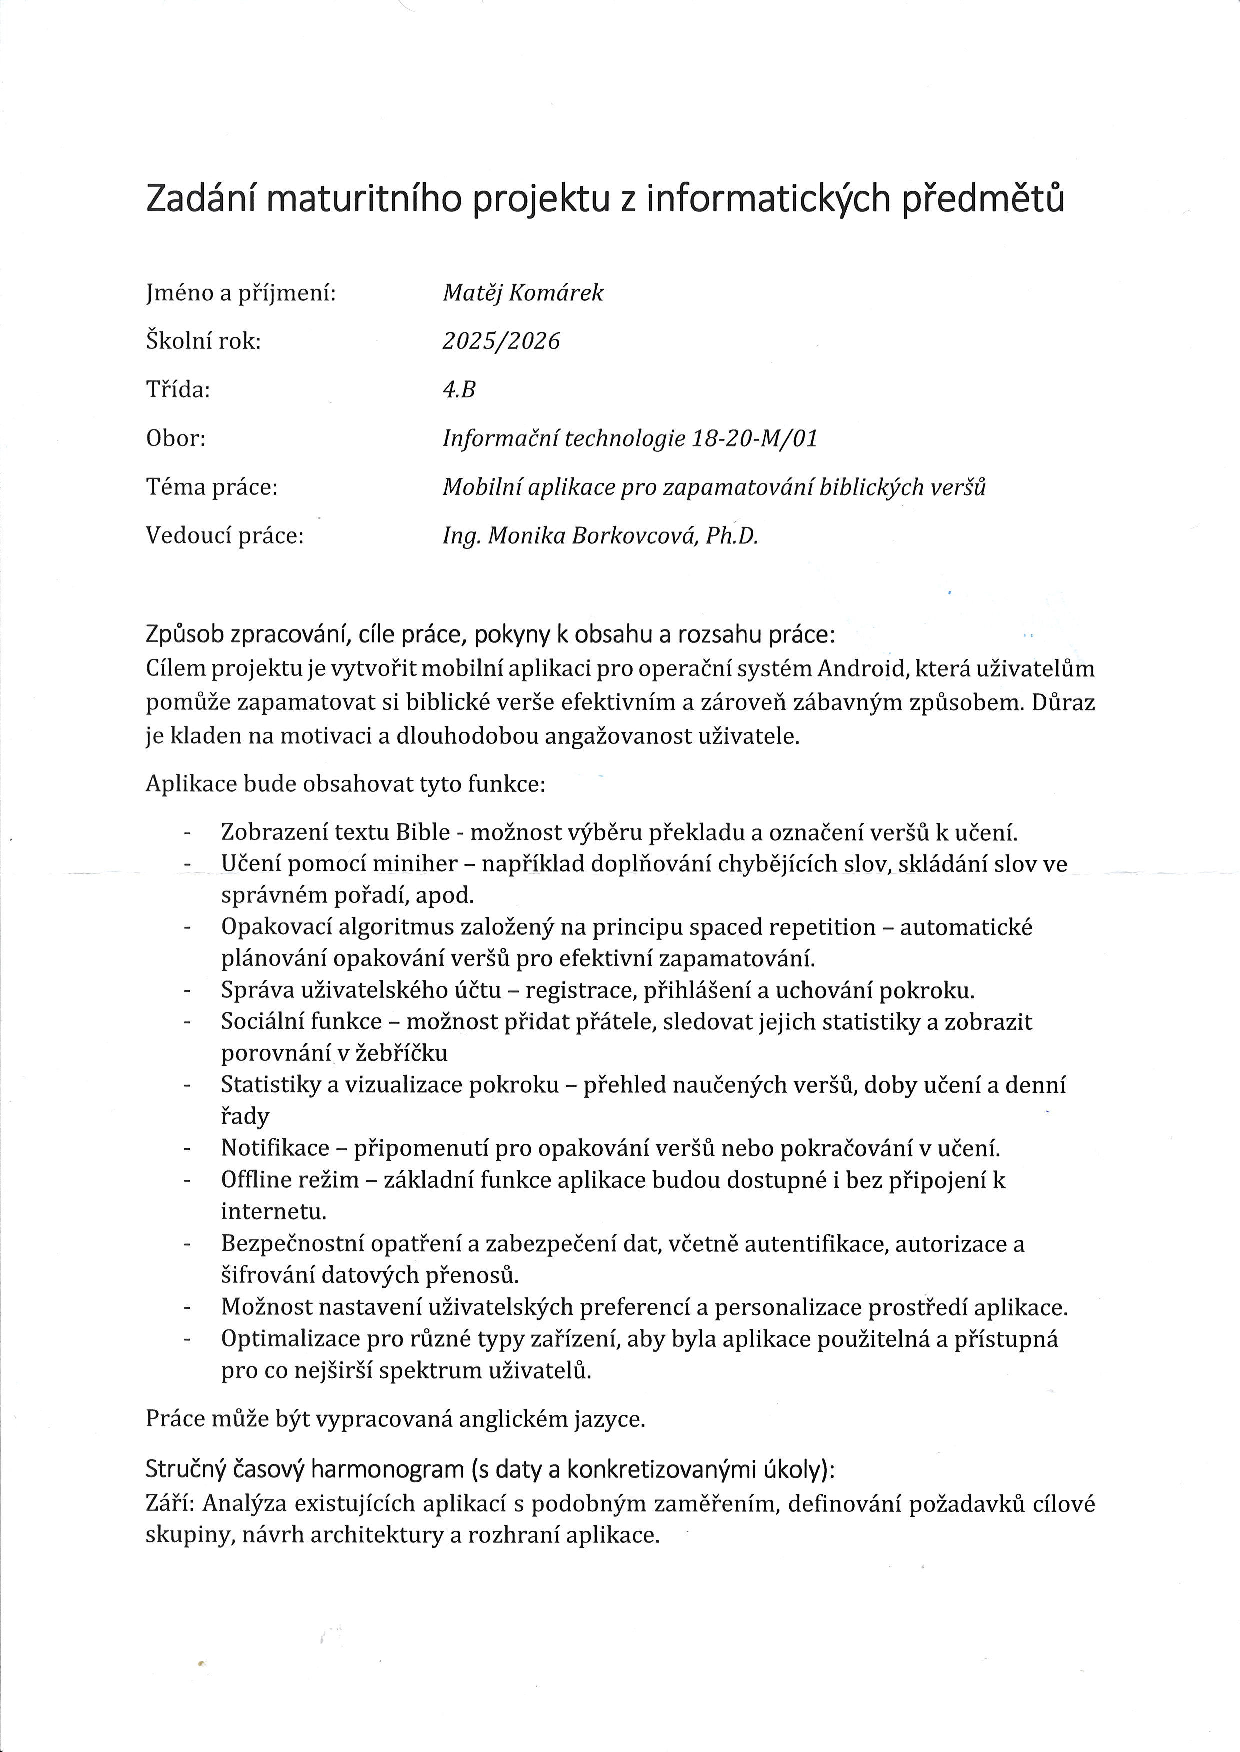
\includepdf[pages={1-2}]{zadani.pdf}


	% 3. Prohlášení
	\newpage
	\thispagestyle{empty}
	
	Prohlašuji, že jsem maturitní projekt vypracoval(a) samostatně, výhradně s použitím uvedené literatury.
		
	\vspace{1cm}
	
	V Pardubicích 30. 3. 2026
	
	\begin{flushright}
		\textit{(vlastnoruční podpis)}
	\end{flushright}
	
	
	% 4. Poděkování
	\newpage
	\thispagestyle{empty}
	\vspace*{12cm}
	
	
	Upřímně děkuji Ing. Monice Borkovcové, Ph.D. jak za odborné vedení a cenné rady při zpracování tohoto projektu, tak za trpělivost a podporu během celé práce.
	
	
	% 5. Resumé a klíčová slova
	\newpage
	\thispagestyle{empty}
	
	\section*{Resumé}
	Práce dokumentuje návrh a vývoj mobilní aplikace Bible Memorizer zaměřené na memorizaci biblických textů. Realizace projektu zahrnuje mobilní aplikaci s podporou offline režimu a backendový server pro synchronizaci a sociální funkce. Mobilní aplikace dále podporuje gamifikaci a učení pomocí intervalového opakování.
	
	% \vspace{2cm}
	
	\section*{Klíčová slova}
	Programování, gamifikace, intervalové opakování, učení, flutter, nestjs, Bible, memorizace
	
	\section*{Abstract}
	This thesis documents the design and development of the Bible Memorizer mobile application, which focuses on the memorization of biblical texts. The implementation of the project includes a mobile application with offline mode support and a backend server for synchronization and social features. Furthermore, the mobile application supports gamification and learning through spaced repetition.
	
	\section*{Keywords}
	Programming, gamification, spaced repetition, learning, flutter, nestjs, Bible, memorization
	
	% 6. Obsah
	\newpage
	\thispagestyle{empty}
	\pagenumbering{gobble}
	\tableofcontents
	
	
	% 7. Odborný text
	\newpage
	\pagenumbering{arabic}
	\setcounter{page}{9}
	
	
	
	\section{Úvod}
	% TODO: Citace na 2.3 miliardy, 8 miliard
	Ve světě žije přes 2.3 miliardy křesťanů, což znamená, že více než čtvrtina lidí jsou křesťané. Častým cílem křesťanů je studium Bible a zapamatování jejich částí.
	Dlouhodobé zapamatování textu ale není jednoduchý úkol.	Existují aplikace, které memorizování částí Bible zjednodušují, ale ty jsou často zastaralé, těžké na používání a neaplikují metody učení, které uživateli pomáhají, urychlují a zpříjemňují celý proces.
	
	Za tímto účelem vznikla aplikace Bible Memorizer. Tato aplikace se snaží jejím uživatelům zjednodušit cíl zapamatování specifických biblických testů. K tomu používá dva hlavní principy. 
	První z nich je gamifikace. Aplikace používá rozmanité minihry, které uživatele přirozeně nutí zastavit se nad daným textem a přemýšlet nad ním novým způsobem.
	
	Druhý princip je intervalové opakování. Intervalové opakování je způsob memorování informace na základě postupně rostoucích intervalů. Díky tomu se uživatelem naučený text uživateli zobrazuje pouze občasně pro kontrolu jeho retence. Uživatel pak nemusí trávit tolik času opakováním veršů, které jsou pro něj jednoduché.
	
	\subsection{Cílová skupina}
	Jak lze z úvodu a celé koncepce projektu jednoduše odvodit, cílovou skupinou této aplikace jsou výhradně křesťané, kteří si chtějí memorizovat biblické verše.
		
	Aplikace však není vázána na specifickou denominaci či církev.
	
	Aplikace zároveň podporuje lokalizaci, díky čemuž umožňuje používání křesťanům z jiných zemí, než jen Česká republika. (Aplikace momentálně podporuje český a anglický jazyk)
	
	\subsection{Terminologie}
	
	\subsubsection{Verš}
	Verš je část textu Bible. Jeho délka je většinou jedna až dvě věty. Jednotlivé verše tvoří kapitoly a jednotlivé kapitoly tvoří biblické knihy, které pak tvoří Bibli.
	
	Každý verš má svojí unikátní, neměnnou referenci většinou udávanou ve formě "název-knihy číslo-kapitoly:číslo-verše". (např. "Jan 3:16")
	
	\subsubsection{Intervalové opakování}
	Intervalové opakování je způsob učení, který se zakládá na postupně rostoucích intervalech. Vysvětleme si to na příkladu. Student se chce naučit nazpaměť jeden verš. První den se ho naučí. Druhý den si ho zopakuje. Třetí den vynechá, ale čtvrtý den se ujistí, že si ho stále pamatuje.
	Tento interval postupně roste, takže student si danou informaci neopakuje každý den. Díky tomu může získaný čas využít na jiné učivo a pojmout tak více informací.
	
	
	% TODO Citace
	% TODO Odkázat se na to v textu
	% https://cs.wikipedia.org/wiki/K%C5%99ivka_zapom%C3%ADn%C3%A1n%C3%AD
	\begin{figure}[htbp]
		\centering
		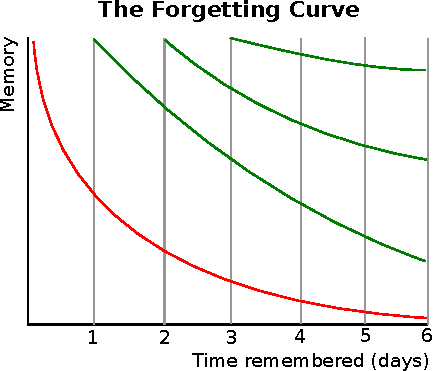
\includegraphics[width=0.8\textwidth]{assets/ForgettingCurve.pdf}
		\caption{Ebbinghausova křivka zapomínání \cite{ebbinghaus_web}}
		\label{fig:krivka}
	\end{figure}

	\section{Analýza existujících řešení}
	V rámci rešerše trhu a mapování konkurenčního prostředí byly podrobně analyzovány čtyři existující mobilní aplikace s obdobným zaměřením. Ačkoliv je primární cíl těchto nástrojů totožný – pomoci uživateli s memorizací textu – analýza odhalila řadu kritických nedostatků, které otevírají prostor pro vytvoření nového, modernějšího řešení.
	
	Zásadním zjištěním je, že většina analyzovaných aplikací nevyužívá pokročilé a vědecky podložené metody učení, jako je například intervalové opakování (spaced repetition). Učení se tak stává méně efektivním. Dalším častým problémem je zastaralé a neintuitivní uživatelské prostředí (UI), které novým uživatelům ztěžuje orientaci a snižuje celkový zážitek z používání (UX).
	
	Z hlediska práce s biblickým textem je častým nedostatkem absence integrované čtečky. Aplikace se často spoléhají na textové pole, do kterého je nutné manuálně zadat přesnou referenci (např. „Jan 3:16“). Tento přístup je náchylný k chybám, uživatelsky nepřívětivý a v jedné z testovaných aplikací byl tento způsob vyhledávání dokonce zcela nefunkční.
	
	Analýza se zaměřila i na motivační a sociální prvky. Pouze jedno z testovaných řešení obsahovalo systém uživatelských žebříčků. Tento systém byl však navržen jako globální a hodnotil uživatele na základě celkového počtu „zapamatovaných“ veršů. Vzhledem k tomu, že stav zapamatování si určuje sám uživatel bez jakéhokoliv objektivního testování, je tento systém snadno zneužitelný a ve výsledku působí spíše demotivačně.
	
	V neposlední řadě představuje velkou bariéru pro tuzemské uživatele absence lokalizace. Žádná z testovaných aplikací nenabízela uživatelské prostředí v českém jazyce a pouze jedna umožňovala stažení českého překladu Bible. Možnosti synchronizace dat byly navíc u většiny aplikací omezené pouze na e-mail, případně na sociální síť Facebook.

	\section{Analýza požadavků}
	Na základě zjištění z analýzy existujících řešení a definování cílové skupiny byly stanoveny konkrétní požadavky na vyvíjenou aplikaci. Tyto požadavky se dělí na funkční, které popisují chování systému, a nefunkční, které definují jeho vlastnosti a kvalitu.
	
	\subsection{Funkční požadavky}
	Systém musí uživatelům poskytovat následující funkcionalitu:
	
	\begin{itemize}
		\item \textbf{Správa uživatelského účtu:} Systém musí umožňovat registraci a přihlášení pomocí účtu Google, odhlášení a kompletní smazání uživatelského účtu i s přidruženými daty.
		\item \textbf{Práce s biblickým textem:} Aplikace musí zobrazovat text Bible s možností plynulého čtení a změny překladu.
		\item \textbf{Správa veršů k memorizaci:} Uživatel musí mít možnost uložit si verš k zapamatování, a to přímým výběrem z textu Bible.
		\item \textbf{Modul učení:} Aplikace musí nabízet procvičování konkrétního vybraného verše i automaticky generovanou sadu doporučených veršů na základě algoritmu intervalového opakování.
		\item \textbf{Zobrazení statistik:} Systém musí uživateli vizualizovat jeho osobní statistiky a postup v učení.
		\item \textbf{Sociální modul:} Uživatelé musí mít možnost přidávat a odebírat přátele (pomocí unikátního kódu), prohlížet si jejich statistiky a porovnávat své výsledky v žebříčku.
		\item \textbf{Personalizace a nastavení:} Aplikace musí umožňovat změnu jazyka rozhraní, přepínání mezi světlým a tmavým motivem (light/dark mode) a úpravu velikosti textu.
	\end{itemize}
	
	\subsection{Nefunkční požadavky}
	Aby byla zajištěna vysoká kvalita a využitelnost softwaru, musí systém splňovat následující kritéria:
	
	\begin{itemize}
		\item \textbf{Výkon a kompatibilita:} Aplikace musí být optimalizována pro plynulý běh i na starších zařízeních, musí podporovat různá rozlišení a poměry stran displeje. Minimální podporovaná verze operačního systému je Android 10.
		\item \textbf{Spolehlivost a dostupnost (Offline režim):} Základní funkce aplikace, jako je prohlížení uložených veršů, hraní miniher a opakování, musí být plně dostupné i bez aktivního připojení k internetu. Uživatelská data se musí automaticky synchronizovat se serverem po obnovení připojení.
		\item \textbf{Bezpečnost:} Veškeré datové přenosy mezi klientem a serverem musí být šifrovány. Systém musí implementovat spolehlivou autentizaci uživatelů a striktní autorizaci pro zajištění bezpečného oddělení dat mezi jednotlivými účty.
		\item \textbf{Použitelnost a přístupnost:} Uživatelské prostředí musí být intuitivní. Důraz je kladen na motivaci a dlouhodobou angažovanost (gamifikace). Aplikace musí být přístupná širokému spektru uživatelů, včetně osob se zhoršeným zrakem (podpora změny velikosti písma).
	\end{itemize}

	\section{Technologie}
	
	\subsection{Flutter}
	Pro vývoj klientské části mobilní aplikace byl zvolen framework Flutter. Jeho klíčovým specifikem pro tento projekt je využití vlastního renderovacího enginu, který generuje nativní uživatelské rozhraní a zajišťuje jeho vizuální i funkční konzistenci napříč různými mobilními zařízeními. Tento přístup eliminuje závislost na nativních UI komponentách jednotlivých operačních systémů, čímž se předchází fragmentaci vzhledu a přispívá k lepší přístupnosti aplikace.
	
	\subsection{NestJS}
	Serverová logika (backend) je implementována pomocí frameworku NestJS. Nástroj vynucuje modulární architekturu, která umožňuje systematické rozdělení aplikace do izolovaných domén. Díky tomuto striktnímu strukturování jsou procesy jako autentizace, autorizace a především synchronizace dat bezpečně odděleny a spravovány, což radikálně snižuje riziko vzniku datových nekonzistencí na straně serveru.
	
	\subsection{PostgreSQL}
	Jako primární databázový systém pro běh na serveru je nasazen PostgreSQL. Slouží k trvalému ukládání relačně strukturovaných entit, mezi které patří uživatelská data, vazby přátelství, historie procvičování a žebříčky. Podpora komplexních relací a striktní dodržování pravidel transakčního zpracování zajišťují absolutní datovou integritu a konzistenci při souběžných aktualizacích a synchronizačních požadavcích od vícera klientů.
	
	\subsection{SQLite}
	Pro správu lokálních dat přímo v paměti mobilního zařízení je využita databáze SQLite. Její implementace je nezbytnou podmínkou pro fungování aplikace v offline režimu. Entitní data o uložených verších, harmonogramu opakování a pokroku v učení jsou ukládána do tohoto lokálního úložiště a následně, po detekci obnoveného síťového připojení, asynchronně synchronizována s hlavní databází na serveru. Uživatel tak neztrácí kontinuitu učení ani při výpadcích sítě.
	
	\subsection{Cloudflare Tunnel}
	Infrastrukturní spojení mezi lokálním serverem a sítí internet zajišťuje démon Cloudflare Tunnel. Tato technologie vytváří šifrované odchozí spojení z aplikačního kontejneru přímo do sítě Cloudflare. Serverová aplikace (NestJS) díky tomu může bezpečně přijímat vnější požadavky bez nutnosti otevírání veřejných portů na serverovém firewallu, konfigurace NAT nebo nutnosti přidělení statické veřejné IP adresy, čímž se minimalizuje povrch pro potenciální síťové útoky.
	
	
	
	\section{Architektura}
	Architektura systému je navržena jako klient-server, kde klientskou část tvoří mobilní aplikace a logiku zpracování dat centralizuje serverová část. Tyto dvě komponenty spolu komunikují převážně asynchronně, aby byla zachována vysoká dostupnost a možnost offline fungování.
	
	% TODO Citace
	% TODO Odkázat se na to v textu
	\begin{figure}[htbp]
		\centering
		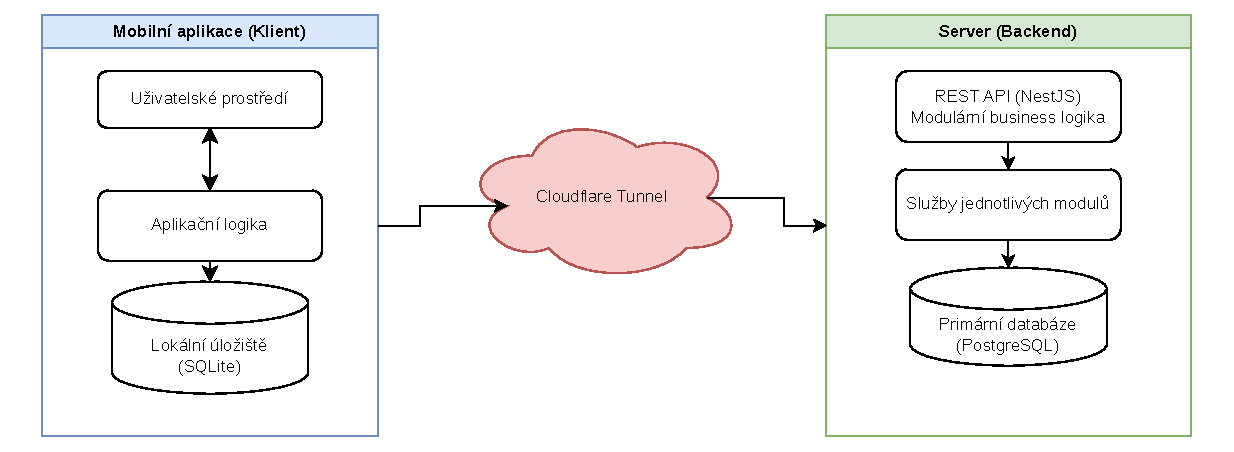
\includegraphics[width=0.8\textwidth]{assets/architecture.pdf}
		\caption{Architektura projektu \cite{ebbinghaus_web}}
		\label{fig:architecture}
	\end{figure}
	
	\subsection{Mobilní aplikace}
	Klientská část je zodpovědná za prezentaci uživatelského rozhraní, lokální vyhodnocování algoritmů a dočasnou perzistenci dat.
	
	\subsubsection{Ukládání dat}
	Lokální ukládání dat v mobilní aplikaci je primárně zajištěno pomocí relační databáze SQLite. Toto řešení je klíčové pro zajištění plnohodnotného běhu aplikace v offline režimu, kdy si uživatel může prohlížet a procvičovat uložené verše bez závislosti na momentálním internetovém připojení. Pro účely následné synchronizace je v lokálním databázovém schématu zavedena vlastnost (\textit{needsSync}), která označuje ty databázové záznamy, jež byly na zařízení nově vytvořeny nebo modifikovány a čekají na odeslání na backend.
	
	\subsubsection{Algoritmy}
	Jádrem logiky aplikace pro plánování učení je implementace principu intervalového opakování (Spaced Repetition). Konkrétně je využit algoritmus SM-2 (SuperMemo-2), který na základě předchozího hodnocení obtížnosti daného verše a zaznamenané úspěšnosti při aktuálním procvičování dynamicky vypočítává datum dalšího opakování. Tímto přístupem dochází k optimalizaci procesu učení – problematické verše jsou uživateli k procvičení předkládány v kratších intervalech, zatímco u dobře osvojených textů se interval do dalšího zobrazení exponenciálně prodlužuje.
	
	\subsection{Server}
	Serverová část aplikačního řešení poskytuje REST API a spravuje primární databázové úložiště. Backend je postaven na frameworku NestJS. Z architektonického hlediska je aplikační kód rozdělen do logických modulů, což umožňuje systematické zapouzdření jednotlivých doménových funkcionalit. Toto modulární členění zajišťuje izolaci business logiky a bezpečné zpracování požadavků.
	
	\subsubsection{Cloudflare Tunnel}
	Pro bezpečné vystavení lokálního serveru do prostředí sítě internet je využit nástroj Cloudflare Tunnel. Tato technologie vytváří zabezpečené odchozí spojení přímo do sítě Cloudflare, čímž eliminuje nutnost otevírání veřejných portů na serverovém firewallu či přiřazování statických veřejných IP adres. Zásadním přínosem tohoto řešení je nativní zajištění šifrované komunikace, kdy je veškerý datový provoz mezi klientskou aplikací a serverem automaticky směrován přes protokol HTTPS, což zaručuje důvěrnost a integritu přenášených dat.
	
	\subsubsection{Synchronizace}
	Synchronizační mechanismus zajišťuje konzistenci dat mezi lokální databází na mobilním zařízení a hlavní serverovou databází. Proces synchronizace je iniciován ze strany klienta. Aplikace vyfiltruje záznamy s vlastností \textit{needsSync} a odešle je formou dávky na server. Pro řešení případných datových konfliktů – například pokud uživatel procvičoval verše offline na dvou různých zařízeních – je implementován mechanismus „zdroje pravdy“ (source of truth) založený na časovém razítku poslední úpravy záznamu. Server při slučování dat porovná časová razítka (\textit{timestamp} nebo datum procvičení) a do hlavní databáze zapíše tu variantu záznamu, která nese nejnovější časový údaj.
	
	\section{Aplikace}
	
	\subsection{Datový model}
	Pro zajištění perzistence dat a spolehlivého chodu aplikace byla navržena robustní databázová architektura. Architektura využívá kombinaci lokální databáze SQLite na mobilním zařízení a centrální relační databáze PostgreSQL na serveru. Následující datový model reflektuje strukturu hlavní serverové databáze.
	
	% TODO Citace
	% TODO Odkázat se na to v textu
	\begin{figure}[htbp]
		\centering
		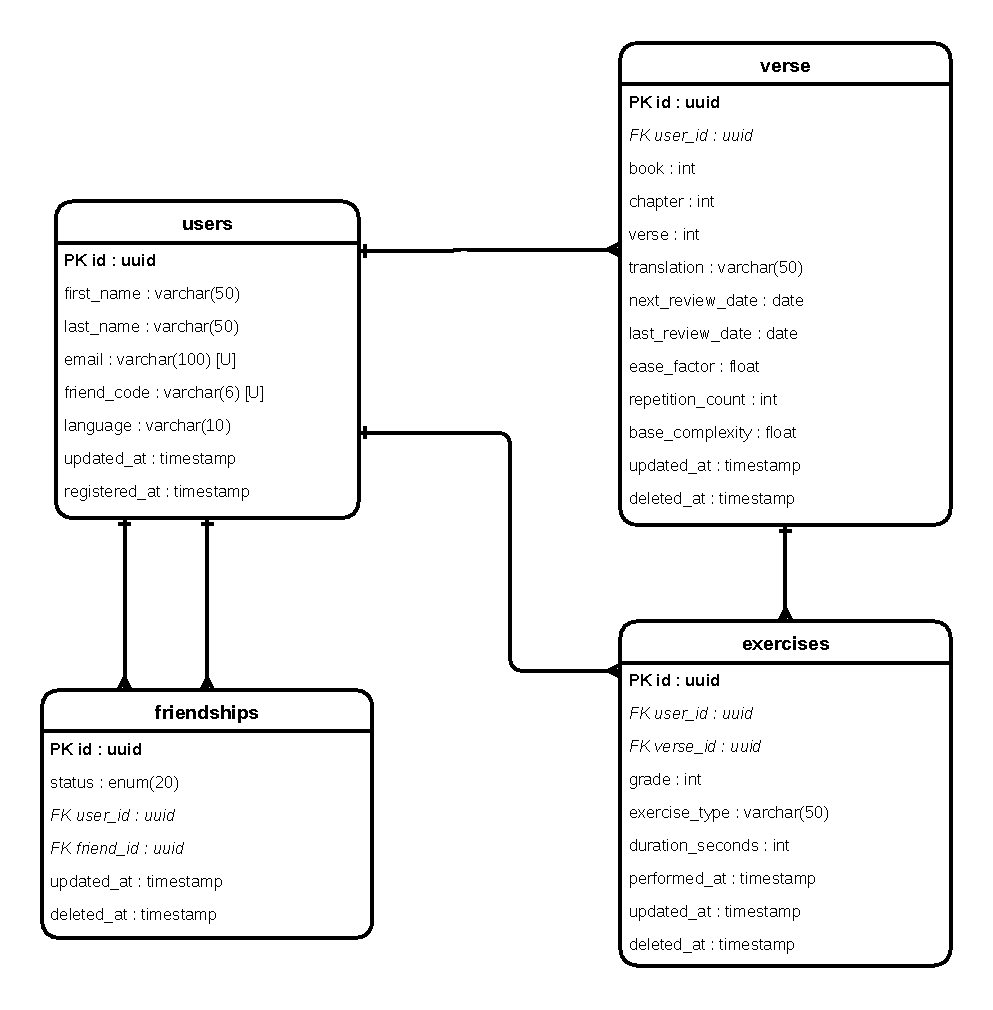
\includegraphics[width=0.8\textwidth]{assets/er.pdf}
		\caption{Datový model \cite{ebbinghaus_web}}
		\label{fig:er}
	\end{figure}
	
	\subsubsection{Entity datového modelu}
	Databázové schéma je rozděleno do čtyř klíčových entit, které reprezentují základní domény aplikace:
	
	\begin{itemize}
		\item \textbf{Uživatel (users):} Centrální entita celého systému. Uchovává identifikační údaje uživatele (jméno, příjmení, e-mail) a jeho osobní preference v aplikaci, jako je zvolený jazyk rozhraní. Dále zaznamenává datum registrace a čas posledního přihlášení. E-mailová adresa slouží jako unikátní identifikátor a nesmí se v systému duplikovat.
		\item \textbf{Uložený verš (saved\_verses):} Entita reprezentující konkrétní biblický text, který si uživatel zvolil k memorizaci. Obsahuje lokační údaje textu (kniha, kapitola, verš) a zvolený překlad. Pro účely intervalového opakování jsou zde uloženy klíčové dynamické atributy: datum posledního procvičení, datum dalšího naplánovaného procvičení a další údaje využívané pro algoritmus intervalového opakování. Každý verš je striktně vázán na právě jednoho uživatele.
		\item \textbf{Procvičení (exercises):} Transakční entita sloužící k logování historie učení. Vzniká při každém dokončení minihry. Zaznamenává časový údaj (timestamp) provedení, celkovou dobu trvání cvičení v sekundách, typ zvolené minihry a hodnotu reprezentující úspěšnost. Záznam je relačně propojen s konkrétním uživatelem a konkrétním uloženým veršem.
		\item \textbf{Přátelství (friendships):} Vazební entita realizující sociální funkce aplikace. Definuje vztah mezi dvěma různými uživateli. Obsahuje stav žádosti. Součástí je také časové razítko vytvoření vazby.
	\end{itemize}
	
	\subsubsection{Zajištění integrity a relace}
	Aby byla zaručena absolutní konzistence dat a ochrana proti anomáliím, využívá databázový model soustavu integritních omezení:
	
	\begin{itemize}
		\item \textbf{Referenční integrita a kaskádové mazání: }Všechny cizí klíče (vazby na uživatele či verše) jsou definovány s pravidlem ON DELETE CASCADE. Pokud je odstraněn uživatelský účet, databáze automaticky a bezpečně odstraní i všechny jeho uložené verše, historii procvičování a vazby přátelství. Tím je zamezeno vzniku tzv. sirotčích záznamů.
		
		\item \textbf{Unikátní omezení: }Tabulka přátelství obsahuje unikátní omezení pro dvojici uživatelů, aby nedocházelo k duplicitním žádostem. Rovněž je pomocí omezující podmínky (Check constraint) zakázáno, aby uživatel odeslal žádost o přátelství sám sobě.
		
		\item \textbf{Ověření domén (Check constraints): }V databázi jsou definována přísná pravidla pro vkládané hodnoty. Číslo kapitoly, číslo verše a délka procvičení musí být vždy kladná čísla.
		\item \textbf{Indexace: }Pro zajištění vysokého výkonu při synchronizaci a vyhledávání jsou nad všemi cizími klíči (např. identifikátor uživatele v tabulce historie) vytvořeny databázové indexy.
	\end{itemize}
	
	\subsection{Bezpečnost}
	Vzhledem k povaze ukládaných uživatelských dat (osobní e-maily, statistiky učení, seznamy přátel) byl kladen vysoký důraz na implementaci adekvátních bezpečnostních opatření, a to jak na straně klientské aplikace, tak na straně serverové infrastruktury.
	
	\subsubsection{Autentizace a ochrana identity}
	Proces ověřování identity uživatelů (autentizace) je řešen výhradně pomocí Google účtu. Tento přístup přenáší odpovědnost za bezpečné ukládání hesel na poskytovatele třetí strany a uživateli nabízí pohodlnější a bezpečnější formu přístupu bez nutnosti vytvářet nové přihlašovací údaje.
	
	Pro sociální funkce (přidávání přátel) byl zaveden systém unikátních šestimístných alfanumerických identifikátorů (Friend Code). Díky tomu je při vyhledávání jiných uživatelů zcela skryta jejich skutečná e-mailová adresa.
	
	\subsubsection{Šifrování a síťová bezpečnost}
	Veškerá komunikace mezi mobilním zařízením a serverem podléhá striktnímu šifrování v průchodu (encryption in transit). Toho je docíleno nasazením technologie Cloudflare Tunnel. Serverová komponenta díky tomuto řešení nemusí mít vystavené veřejné porty, čímž se drasticky snižuje riziko přímého útoku na infrastrukturu. Veškerý datový provoz je tak nuceně směrován přes zabezpečený protokol HTTPS, který zajišťuje důvěrnost a zabraňuje zachycení komunikace.
	
	\subsubsection{Autorizace a ochrana dat}
	Serverová architektura postavená na frameworku NestJS využívá propracovaný systém kontrolerů a guardů (ochranných vrstev). Ty zajišťují, že každý požadavek směřující na aplikační programové rozhraní (API) je podroben kontrole přístupových práv. Uživatel může prostřednictvím synchronizačních endpointů číst, upravovat či odstraňovat výhradně ty databázové záznamy, které jsou jednoznačně přiřazeny k jeho vlastnímu identifikačnímu číslu (userId). Jakýkoliv pokus o manipulaci s daty jiných uživatelů je serverem automaticky zamítnut.
	
	
	
	
	\subsection{Dokumentace API rozhraní}
	
	Backendová část aplikace postavená na frameworku NestJS poskytuje REST API, které je navrženo pro efektivní synchronizaci dat a správu uživatelských profilů. Veškerá komunikace (s výjimkou systémových endpointů) vyžaduje autentizaci pomocí JWT tokenu.
	
	\subsubsection{Synchronizační endpointy (SyncController)}
	Tyto endpointy tvoří jádro aplikace a umožňují dávkové (batch) zpracování dat pro zajištění plynulého offline režimu.
	
	\begin{itemize}
		\item \textbf{GET /sync/pull}
		\begin{itemize}
			\item \textbf{Popis:} Slouží k získání dat ze serveru směrem do klientské aplikace od času poslední úspěšné synchronizace.
			\item \textbf{Vstupní parametry (Query):} \texttt{lastSync} (String, ISO datum – čas poslední úspěšné synchronizace).
			\item \textbf{Návratová hodnota:} JSON objekt obsahující \texttt{timestamp} (aktuální čas serveru) a objekt \texttt{changes} se seznamy nových či upravených entit (\texttt{verses}, \texttt{exercises}, \texttt{friendships}, \texttt{user}).
		\end{itemize}
		
		\item \textbf{POST /sync/push}
		\begin{itemize}
			\item \textbf{Popis:} Zajišťuje nahrání lokálních změn z klientského zařízení na server.
			\item \textbf{Vstupní parametry (Body):} JSON objekt \texttt{SyncPushDto} obsahující pole entit k uložení nebo aktualizaci (\texttt{verses}, \texttt{exercises}, \texttt{friendships}, \texttt{user}).
			\item \textbf{Návratová hodnota:} Objekt potvrzující úspěšné zpracování požadavku: \texttt{\{ "success": true \}}.
		\end{itemize}
	\end{itemize}
	
	\subsubsection{Uživatelské endpointy (UserController)}
	Tento kontroler spravuje operace vázané na uživatelský profil, sociální interakce a výpočet pokroku.
	
	\begin{itemize}
		\item \textbf{POST /user/login}
		\begin{itemize}
			\item \textbf{Popis:} Slouží k autentizaci uživatele a inicializaci jeho profilu v databázi. Pokud uživatel v systému neexistuje, je mu automaticky vytvořen účet a přidělen unikátní kód přátelství (\texttt{friendCode}).
			\item \textbf{Zabezpečení:} Chráněno pomocí \texttt{AuthGuard('jwt-login')}.
			\item \textbf{Návratová hodnota:} Kompletní objekt uživatele (\texttt{User}).
		\end{itemize}
		
		\item \textbf{GET /user/lookup}
		\begin{itemize}
			\item \textbf{Popis:} Endpoint pro vyhledávání uživatelů za účelem navázání přátelství na základě unikátního kódu.
			\item \textbf{Vstupní parametry (Query):} \texttt{friendCode} (String, šestimístný alfanumerický identifikátor).
			\item \textbf{Návratová hodnota:} Veřejný profil uživatele obsahující \texttt{id}, \texttt{firstName} a \texttt{lastName}.
		\end{itemize}
		
		\item \textbf{GET /user/:id/stats}
		\begin{itemize}
			\item \textbf{Popis:} Slouží k asynchronnímu výpočtu a zobrazení komplexních uživatelských statistik.
			\item \textbf{Vstupní parametry (Param):} \texttt{id} (identifikátor uživatele).
			\item \textbf{Návratová hodnota:} Objekt statistik zahrnující \texttt{streak} (aktuální denní řada), \texttt{totalPractices} (celkový počet procvičení), \texttt{memorizedVerses} (počet zapamatovaných veršů na základě úspěšnosti), \texttt{timeSpentSeconds} (celkový čas strávený učením) a \texttt{score} (bodové hodnocení aktivity).
		\end{itemize}
		
		\item \textbf{DELETE /user/me}
		\begin{itemize}
			\item \textbf{Popis:} Zajišťuje kompletní a bezpečné odstranění uživatelského účtu včetně všech navázaných dat (veršů, procvičení i přátelství) v rámci jedné transakce pro zachování integrity databáze.
			\item \textbf{Návratová hodnota:} \texttt{\{ "success": true \}}.
		\end{itemize}
	\end{itemize}
	
	\subsubsection{Systémové endpointy (AppController)}
	\begin{itemize}
		\item \textbf{GET /health}
		\begin{itemize}
			\item \textbf{Popis:} Standardní endpoint pro monitorování dostupnosti a životního cyklu aplikačního kontejneru.
			\item \textbf{Návratová hodnota:} \texttt{\{ "status": "ok" \}}.
		\end{itemize}
	\end{itemize}
	
	
	
	\subsection{Uživatelské rozhraní}
	Vzhledem ke zjištěním z úvodní rešerše byl při návrhu klientské části kladen extrémní důraz na použitelnost, přístupnost a dlouhodobou motivaci uživatele. Uživatelské rozhraní (UI) bylo navrženo tak, aby bylo intuitivní a minimalizovalo kognitivní zátěž při každodenním používání.
	
	\begin{figure}[H]
		\centering
		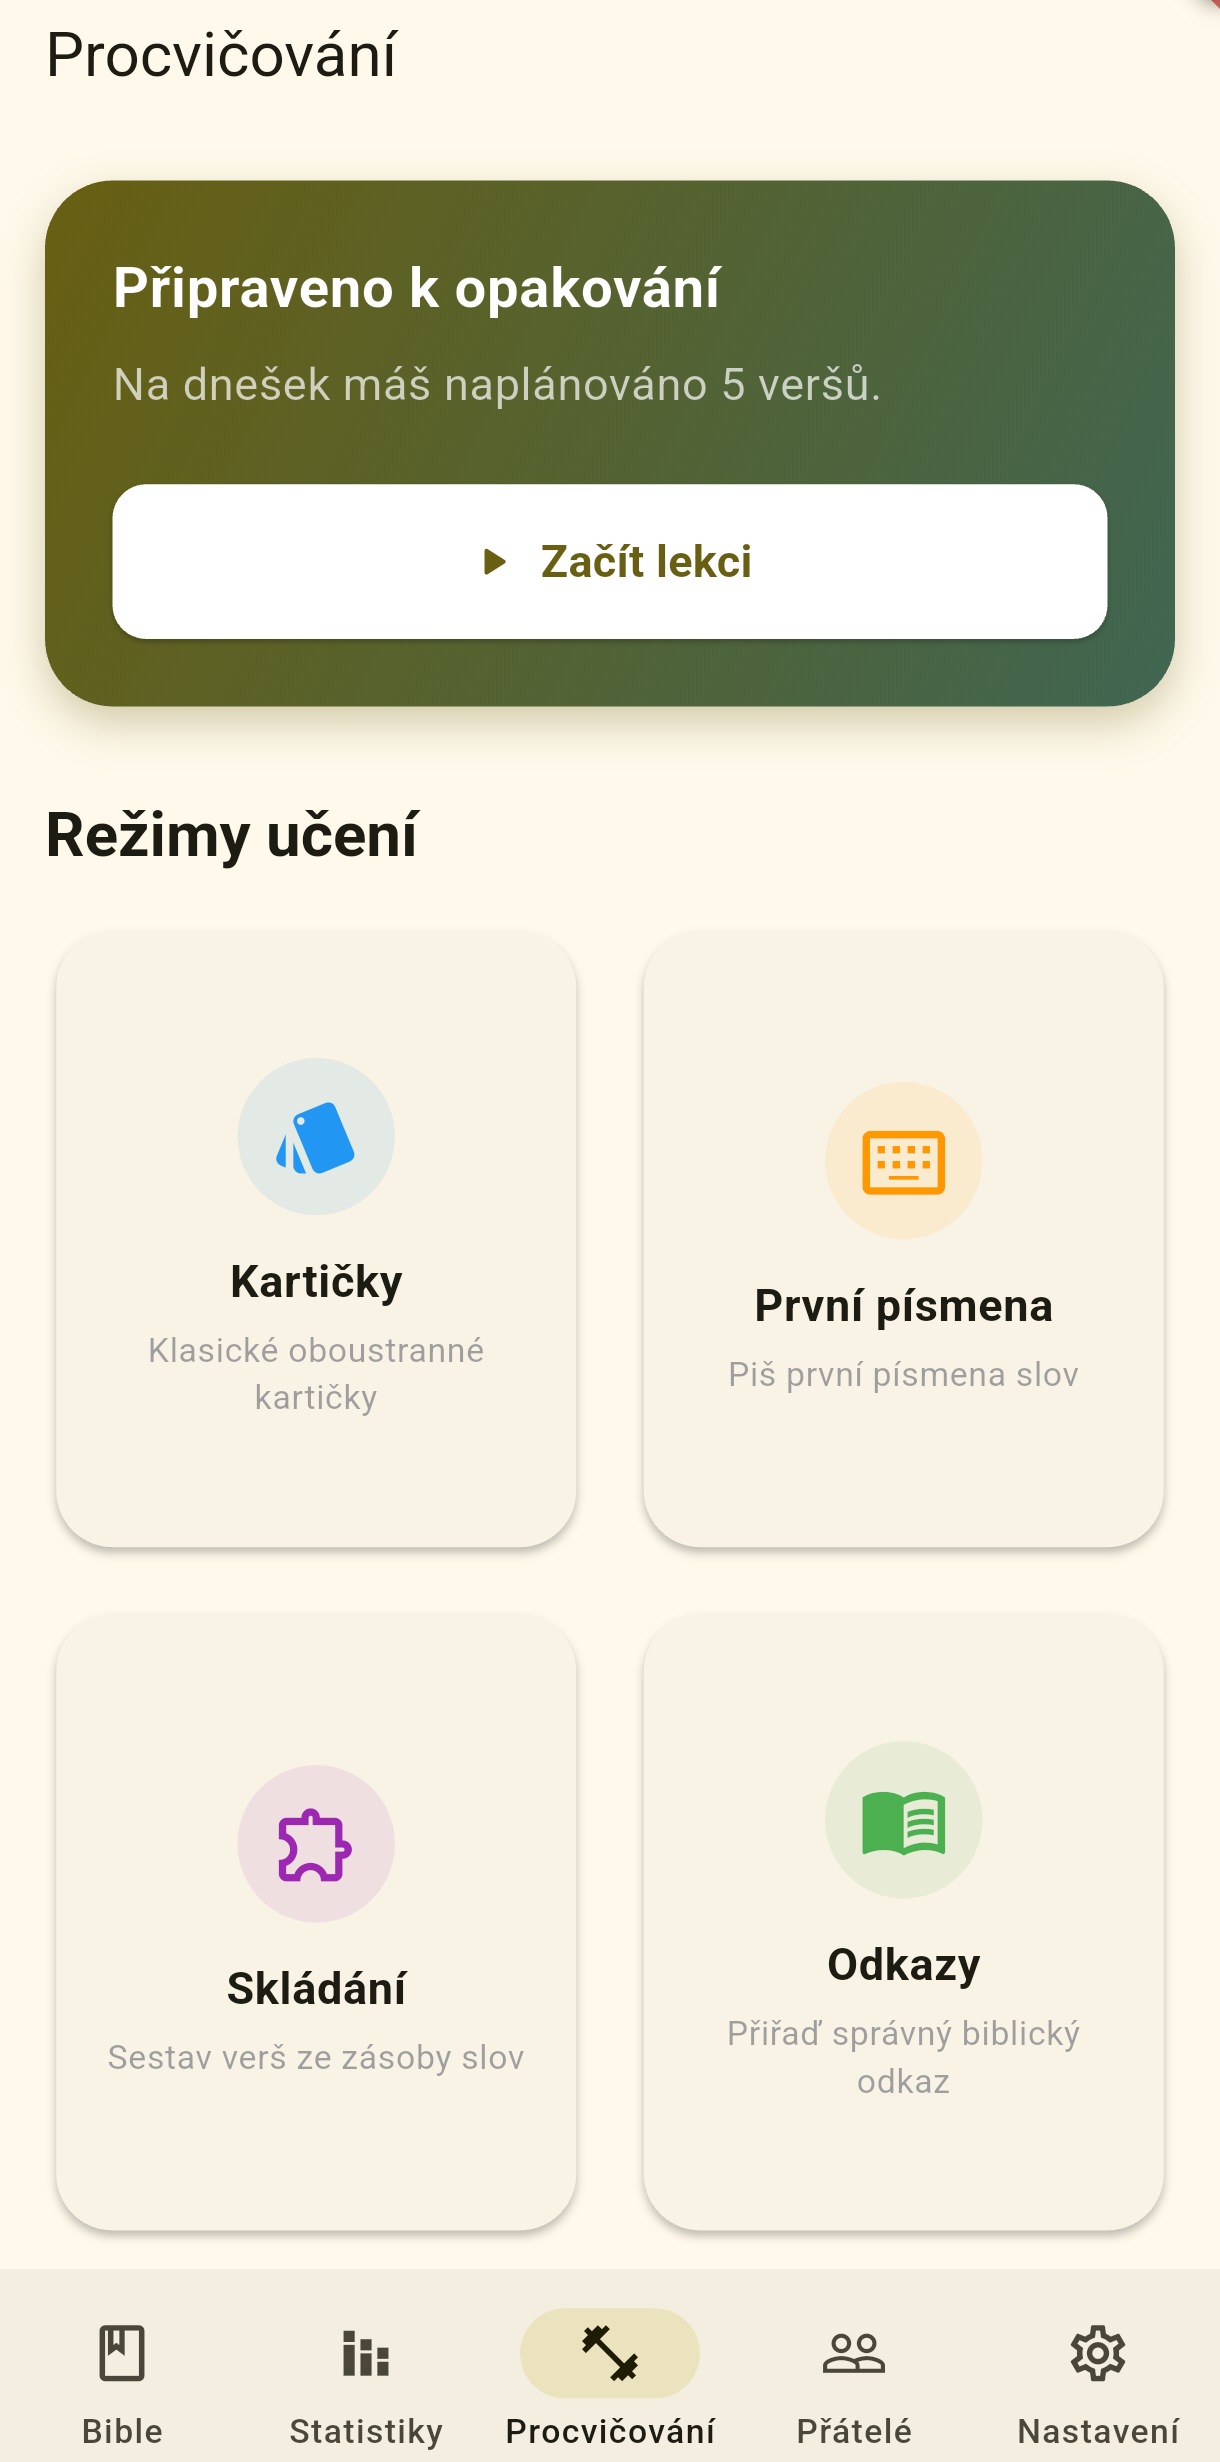
\includegraphics[height=12cm]{assets/screenshots/home.png}
		\caption{Hlavní obrazovka aplikace}
	\end{figure}
	
	\subsubsection{Přístupnost a personalizace}
	Aby aplikace vyhovovala co nejširšímu spektru uživatelů, včetně osob se specifickými potřebami, obsahuje systém několik úrovní personalizace:
	\begin{itemize}
		\item \textbf{Vizuální motivy:} Systém nativně podporuje přepínání mezi světlým (light mode) a tmavým (dark mode) motivem. Tmavý motiv snižuje únavu očí při používání aplikace ve zhoršených světelných podmínkách.
		\item \textbf{Velikost typografie:} Aplikace nabízí možnost uživatelsky upravit velikost zobrazovaného textu. Tato funkce je kritická pro zajištění přístupnosti uživatelům se zhoršeným zrakem, čímž je naplněn jeden z hlavních nefunkčních požadavků.
		\item \textbf{Lokalizace:} Prostředí aplikace je plně lokalizováno. Uživatel si může v nastavení zvolit preferovaný jazyk uživatelského rozhraní, což odstraňuje bariéry pro neanglicky mluvící uživatele.
	\end{itemize}
	
	\begin{figure}[H]
		\centering
		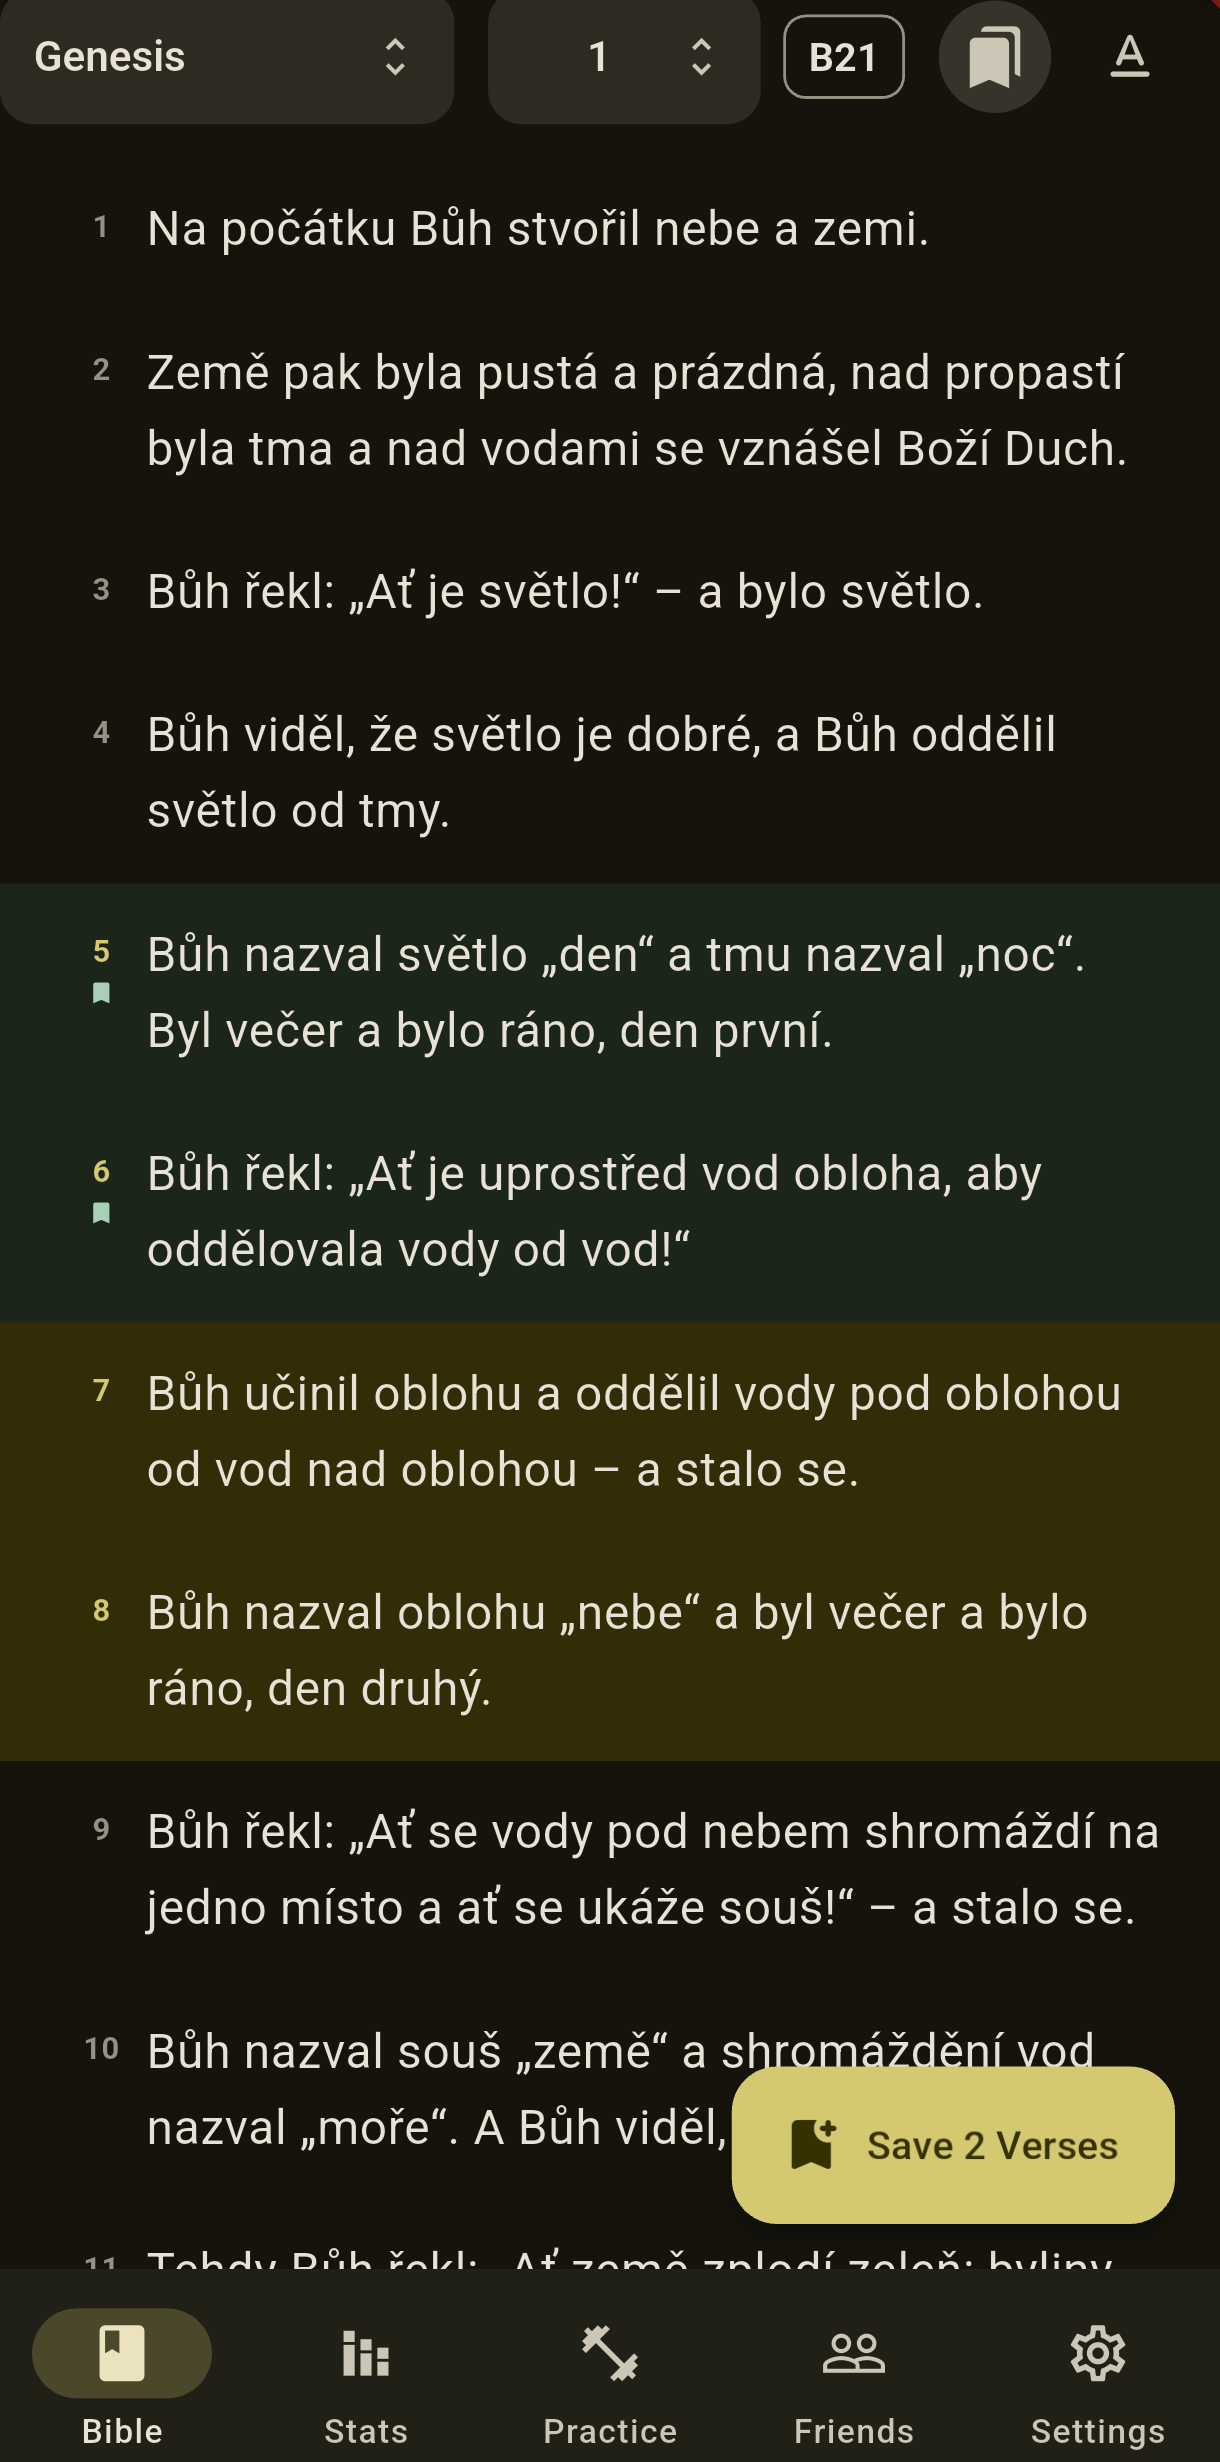
\includegraphics[height=12cm]{assets/screenshots/dark.png}
		\hspace{1cm} % Mezera mezi obrázky
		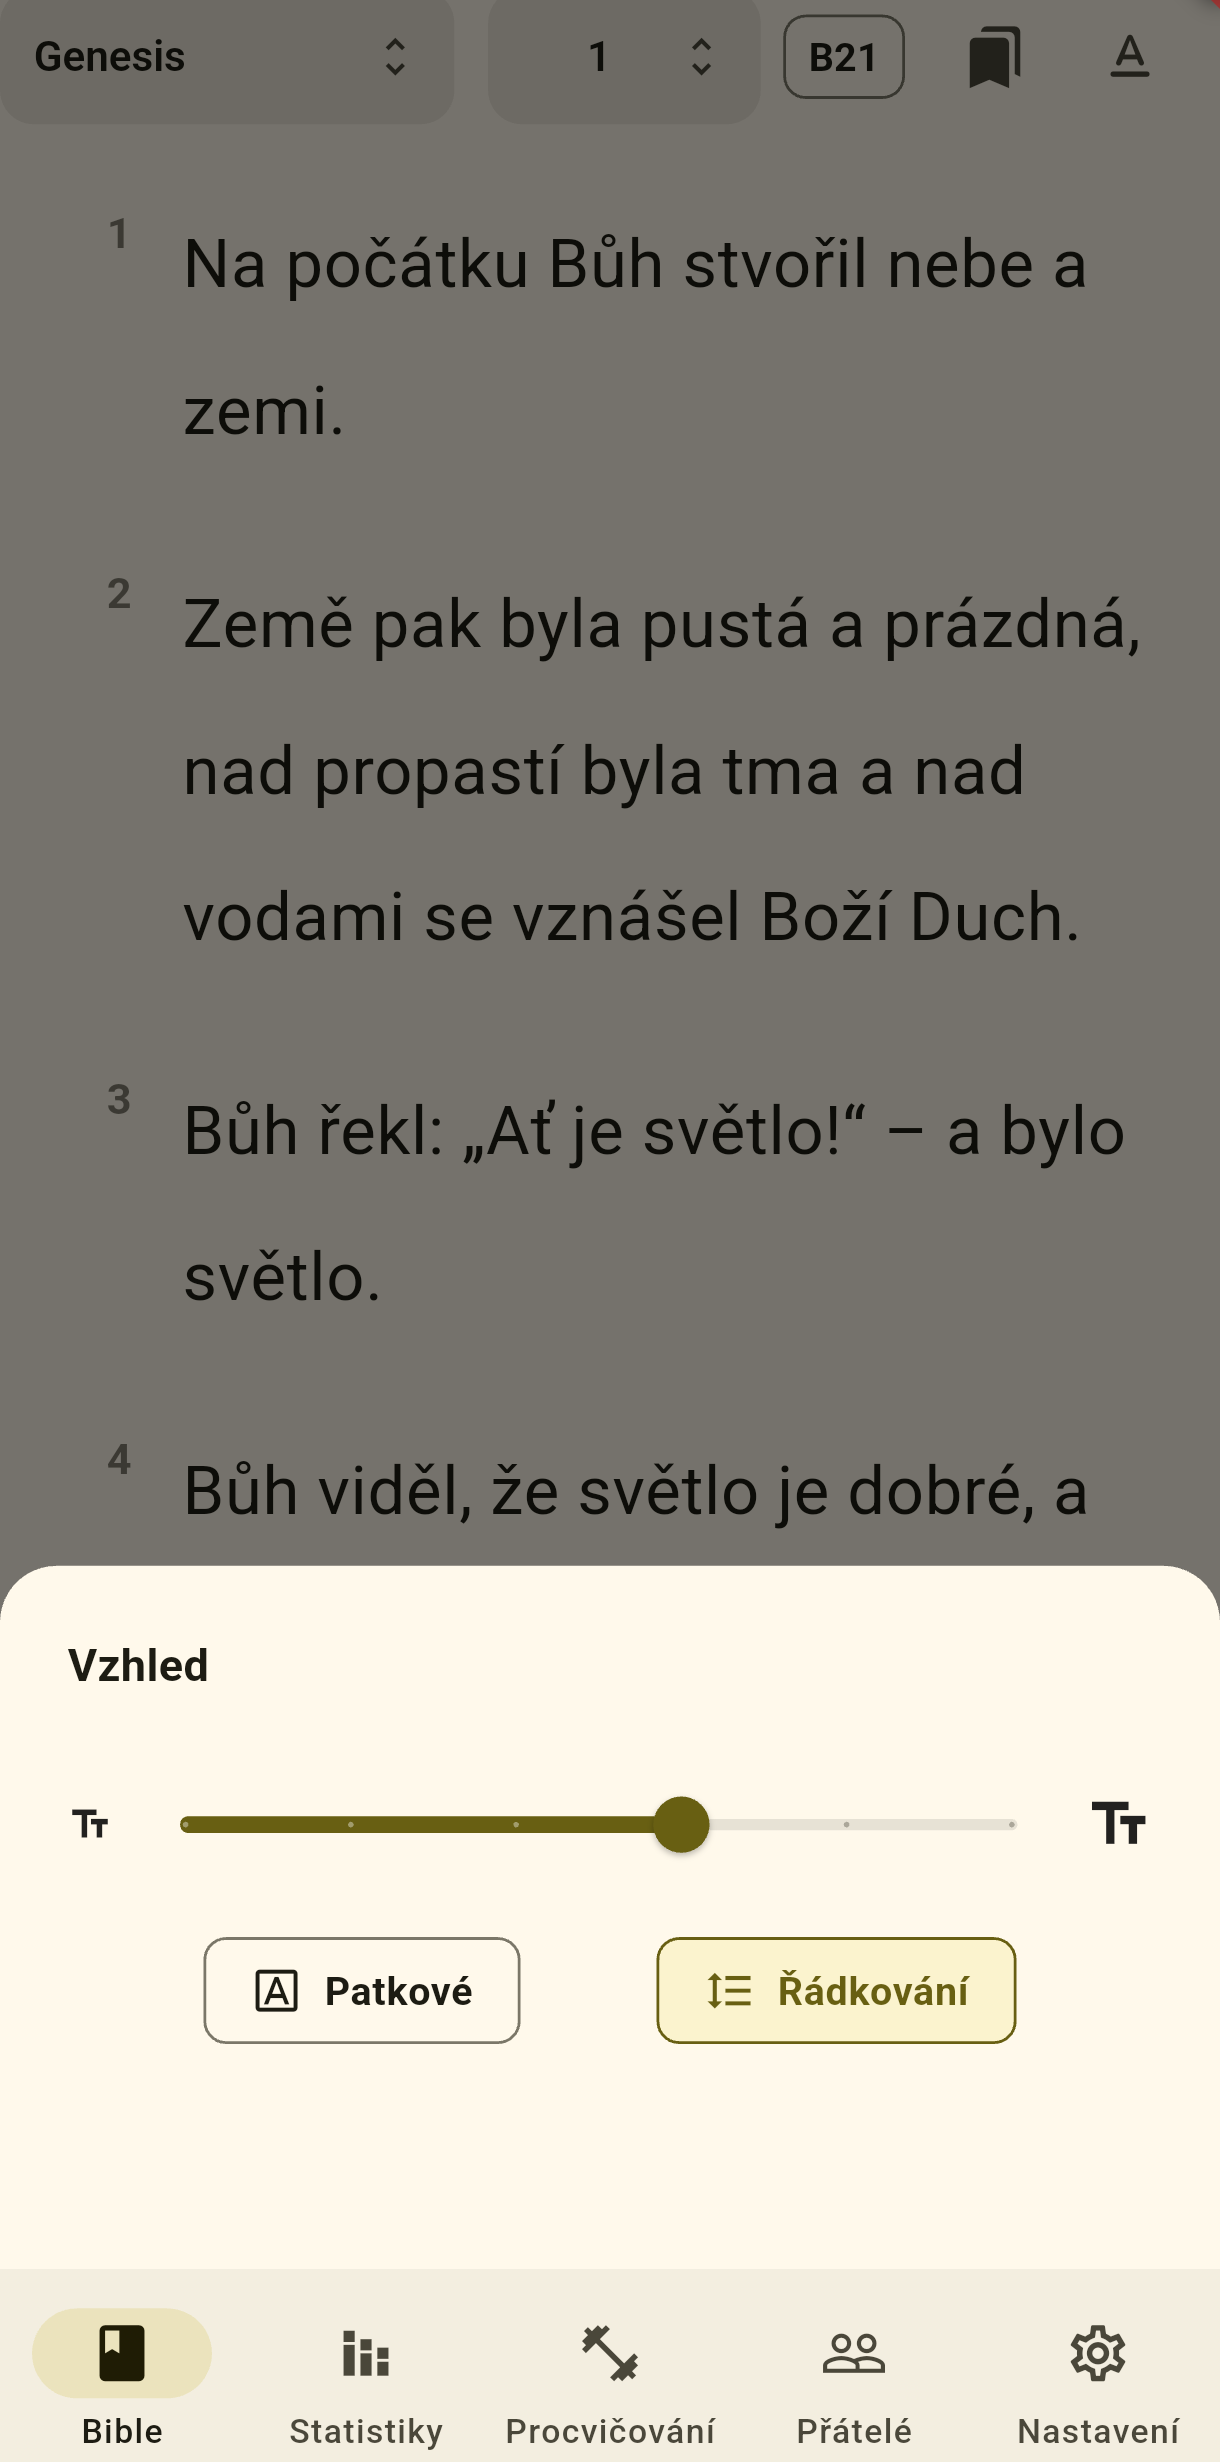
\includegraphics[height=12cm]{assets/screenshots/text-size.png}
		\caption{Tmavý motiv a přizpůsobení velikosti textu}
	\end{figure}
	
	\subsection{Gamifikace a motivační prvky}
	Samotný proces memorizace textu je kognitivně náročný. Pro zvýšení retence (udržení uživatele v aplikaci) byly implementovány prvky gamifikace, které proces učení transformují do poutavější formy:
	
	\begin{itemize}
		\item \textbf{Minihry pro učení:} Namísto pouhého pasivního čtení textu je procvičování realizováno formou interaktivních miniher. Uživatel je například vyzván k doplňování chybějících slov nebo k sestavování frází ve správném pořadí. Tento přístup nutí uživatele nad textem aktivně přemýšlet.
		
		\begin{figure}[H]
			\centering
			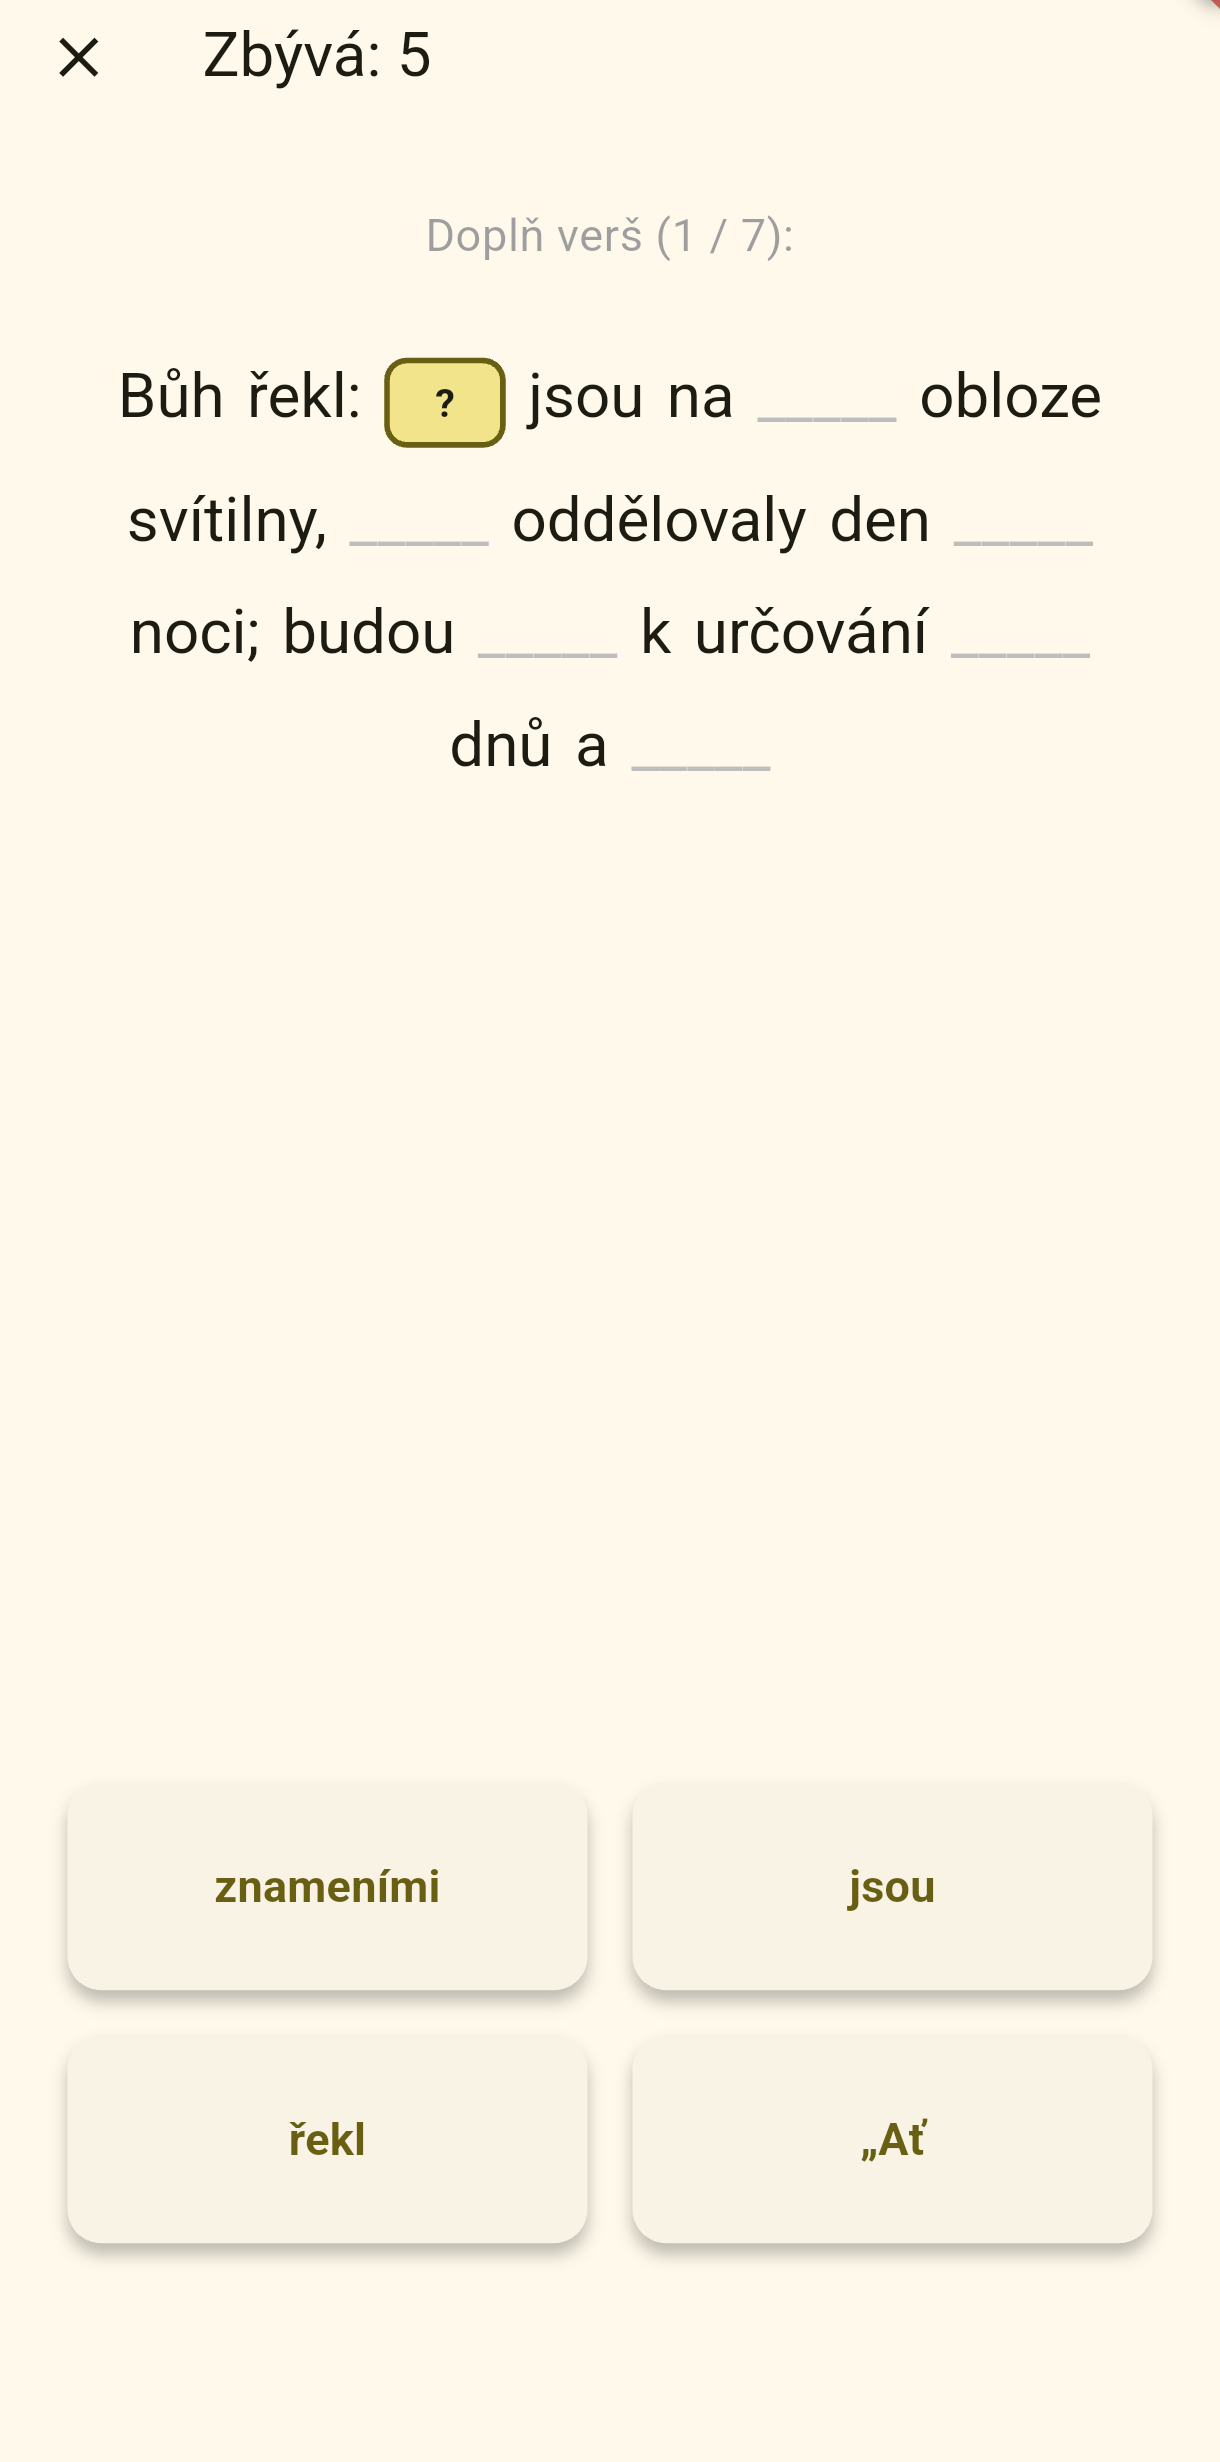
\includegraphics[height=12cm]{assets/screenshots/word-pick.png}
			\hspace{0.5cm}
			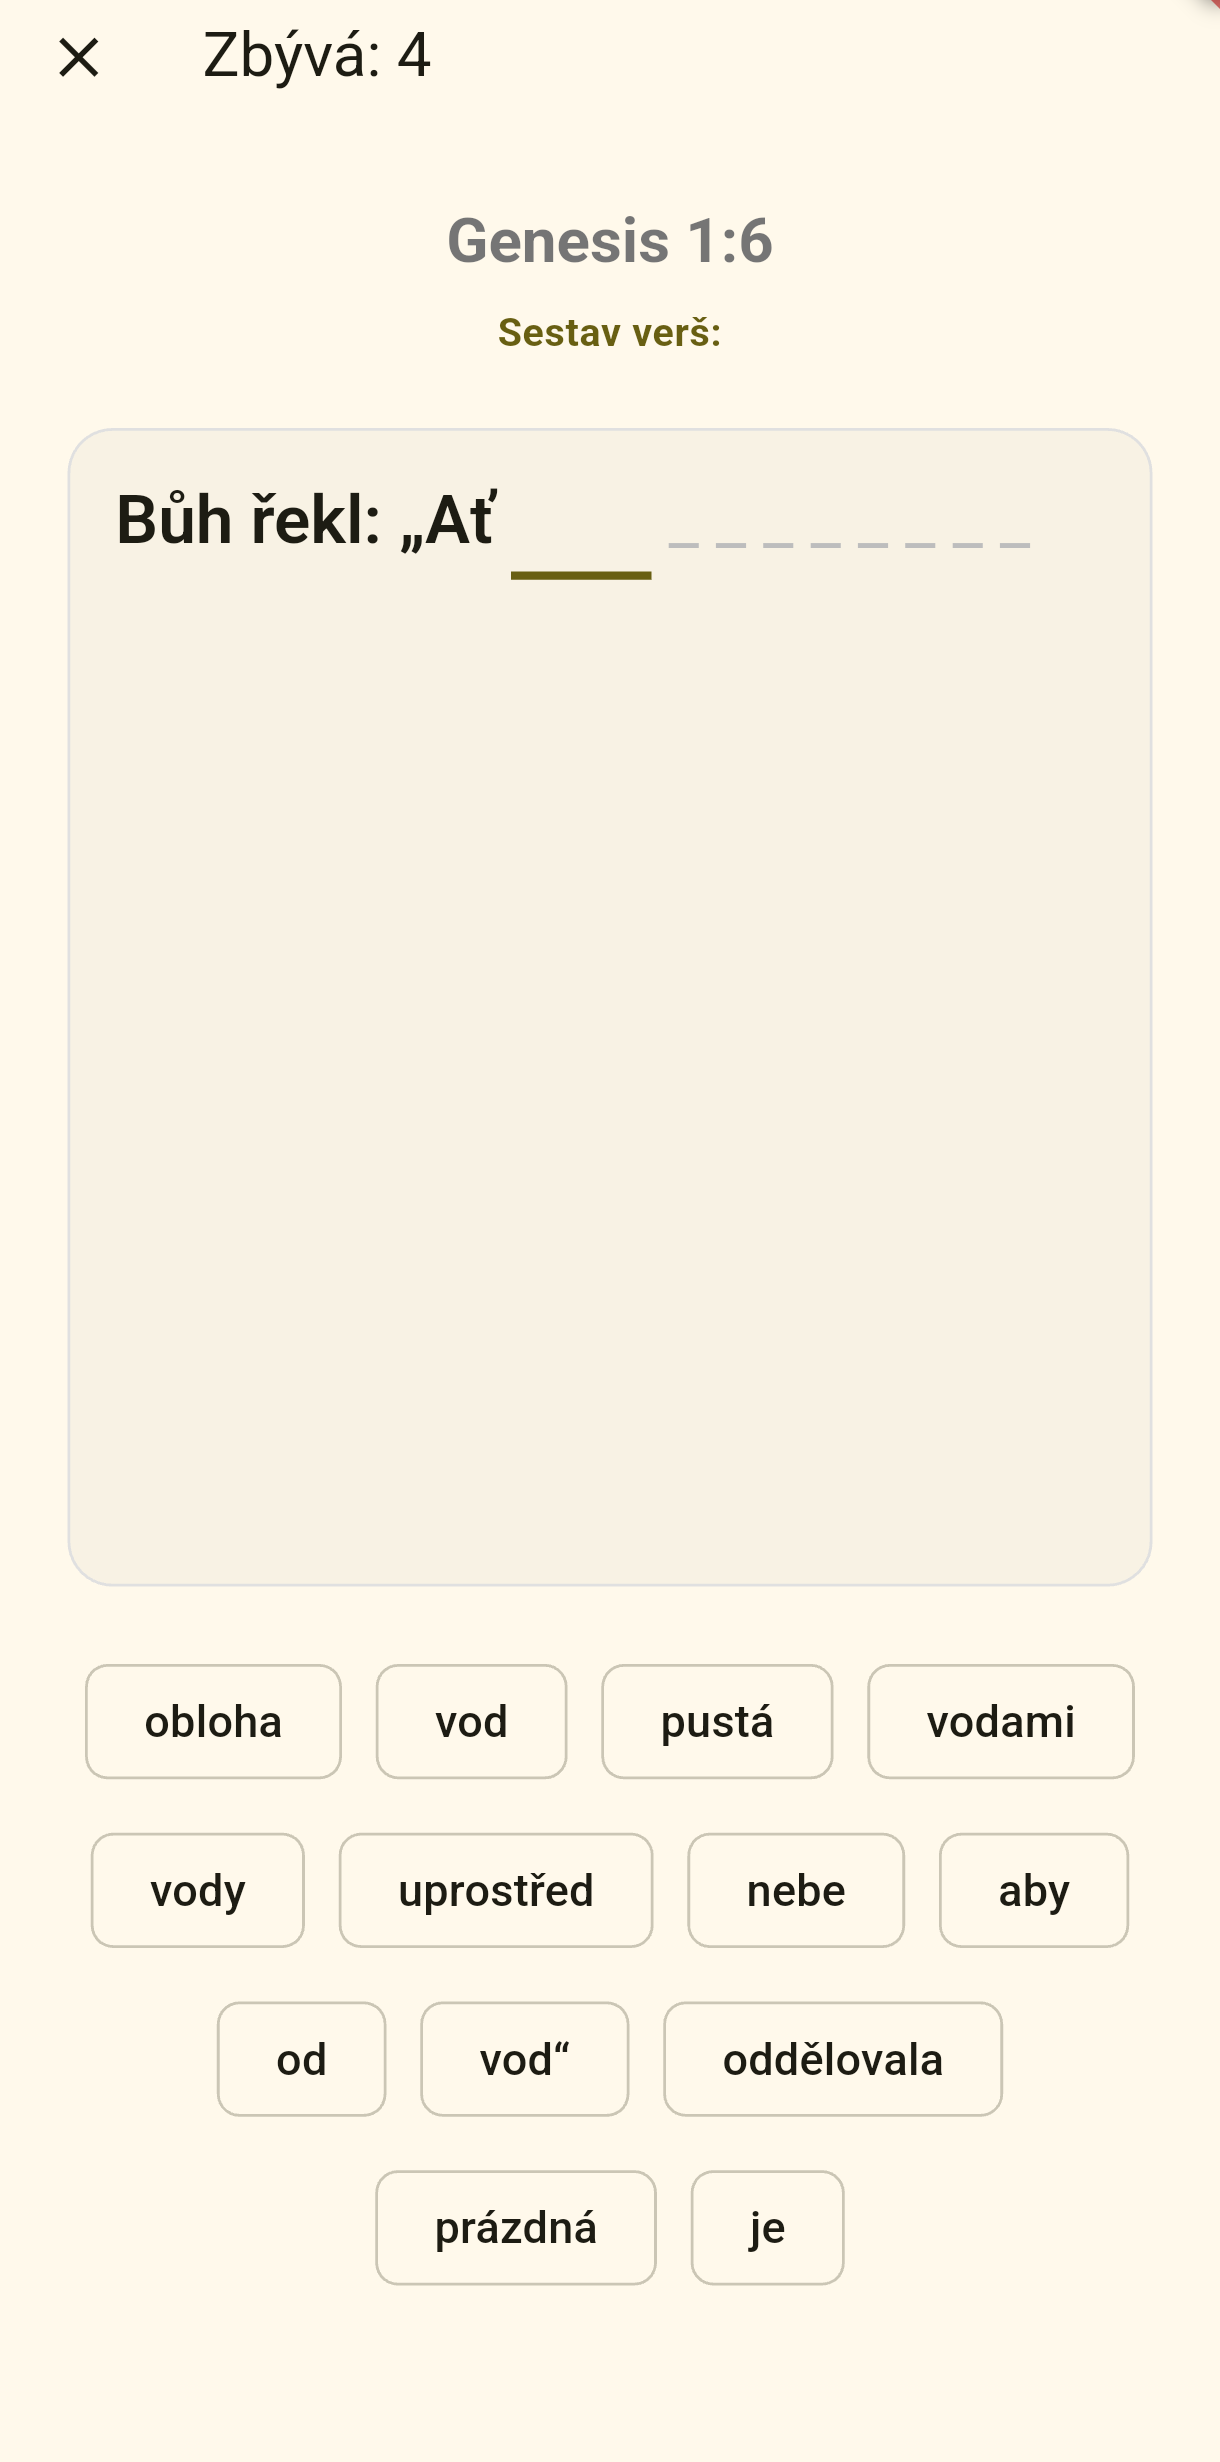
\includegraphics[height=12cm]{assets/screenshots/skladani.png} \\
			\vspace{0.5cm} % Mezera mezi horní a dolní řadou
			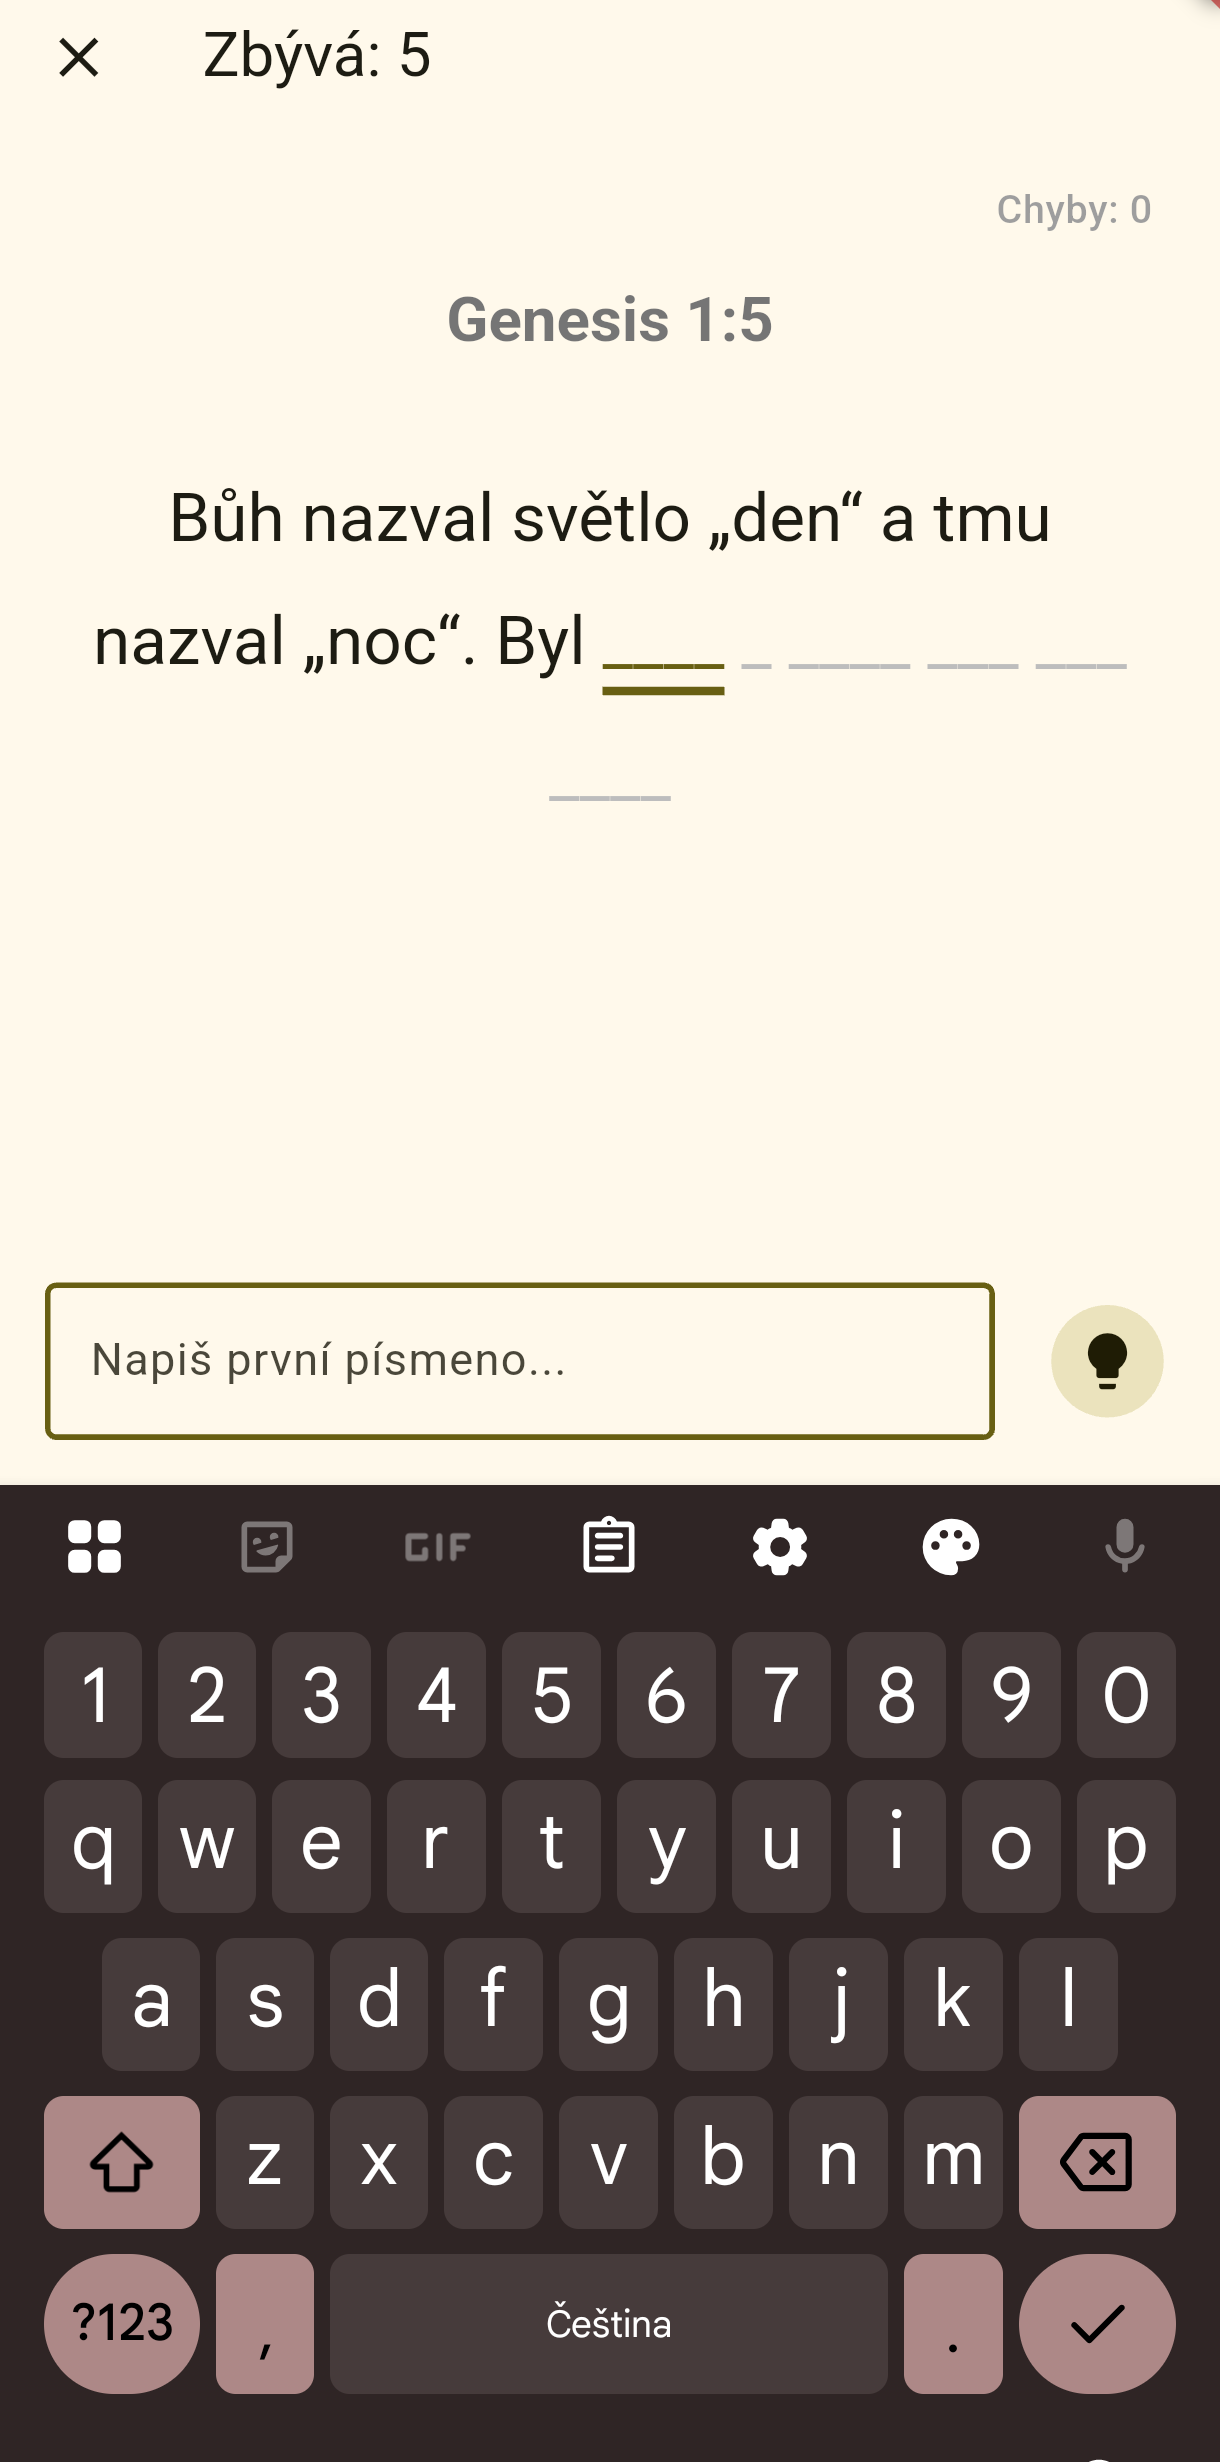
\includegraphics[height=12cm]{assets/screenshots/first-letter.png}
			\hspace{0.5cm}
			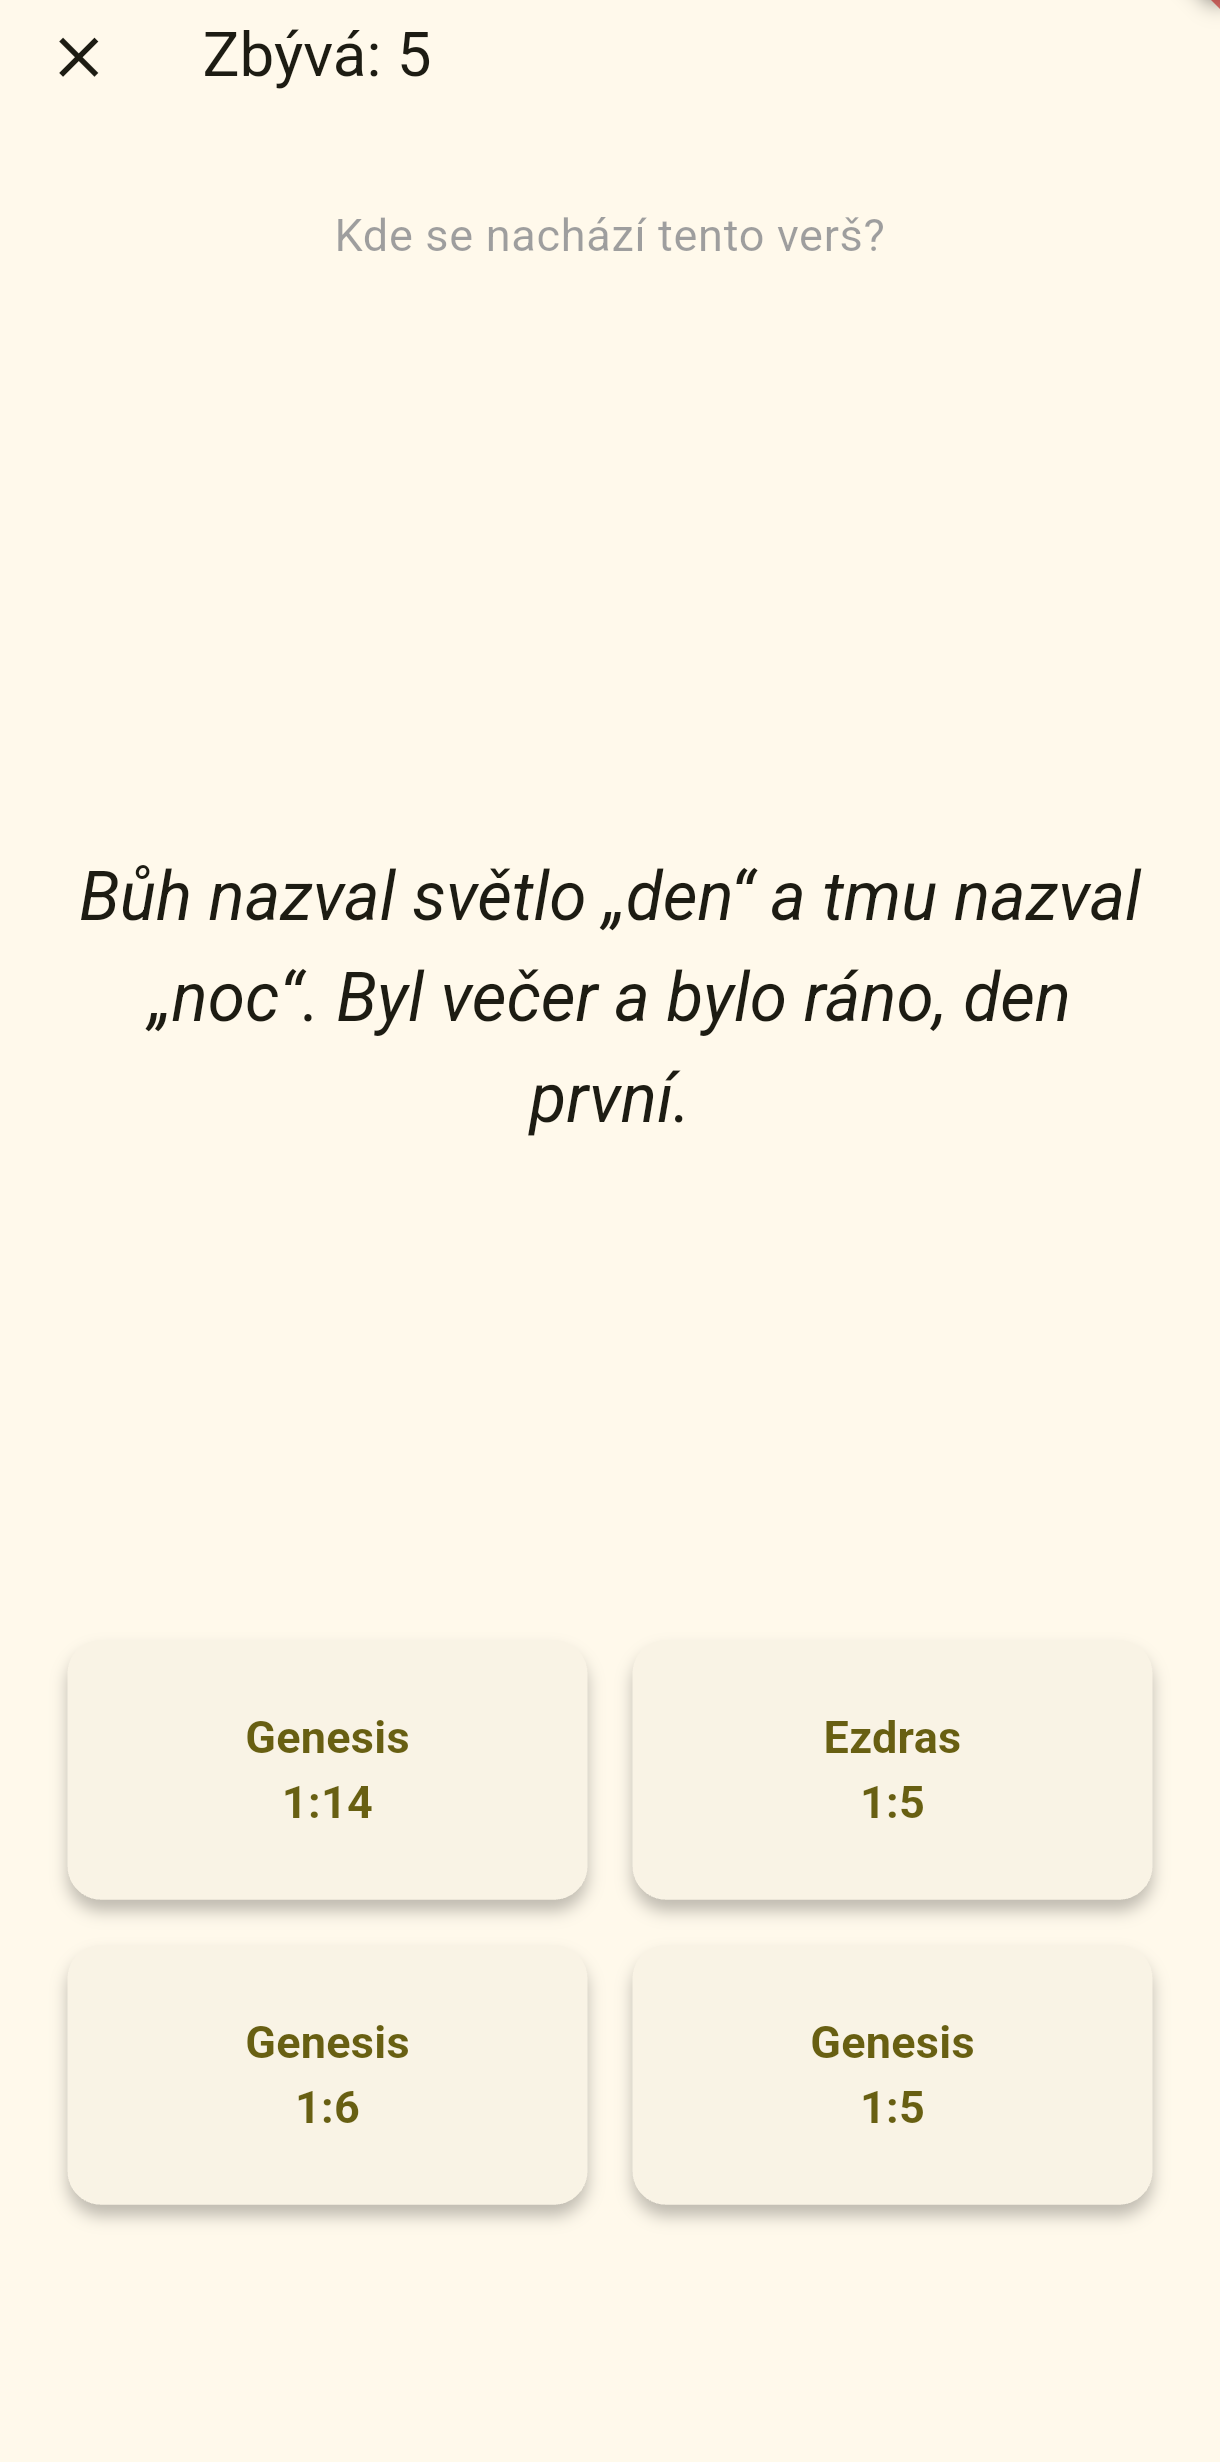
\includegraphics[height=12cm]{assets/screenshots/reference.png}
			\caption{Ukázka interaktivních miniher a výběru veršů}
			\label{fig:minihry}
		\end{figure}
		
		\item \textbf{Sledování denní řady (Streak):} Aplikace vizualizuje konzistenci uživatele pomocí denní řady. Každý den, kdy uživatel úspěšně splní naplánované opakování, se jeho řada prodlužuje. Tento psychologický prvek silně motivuje k pravidelnému návratu do aplikace.
		\item \textbf{Sociální interakce a žebříčky:} Prostřednictvím unikátního kódu přátelství (Friend Code) se mohou uživatelé propojovat. Osobní statistiky a postup v učení jsou následně vizualizovány a porovnávány v lokálních žebříčcích mezi přáteli. Na rozdíl od konkurenčních řešení je tento systém spravedlivější, neboť hodnotí reálnou aktivitu (např. čas strávený učením a udrženou denní řadu).
		
		\begin{figure}[H]
			\centering
			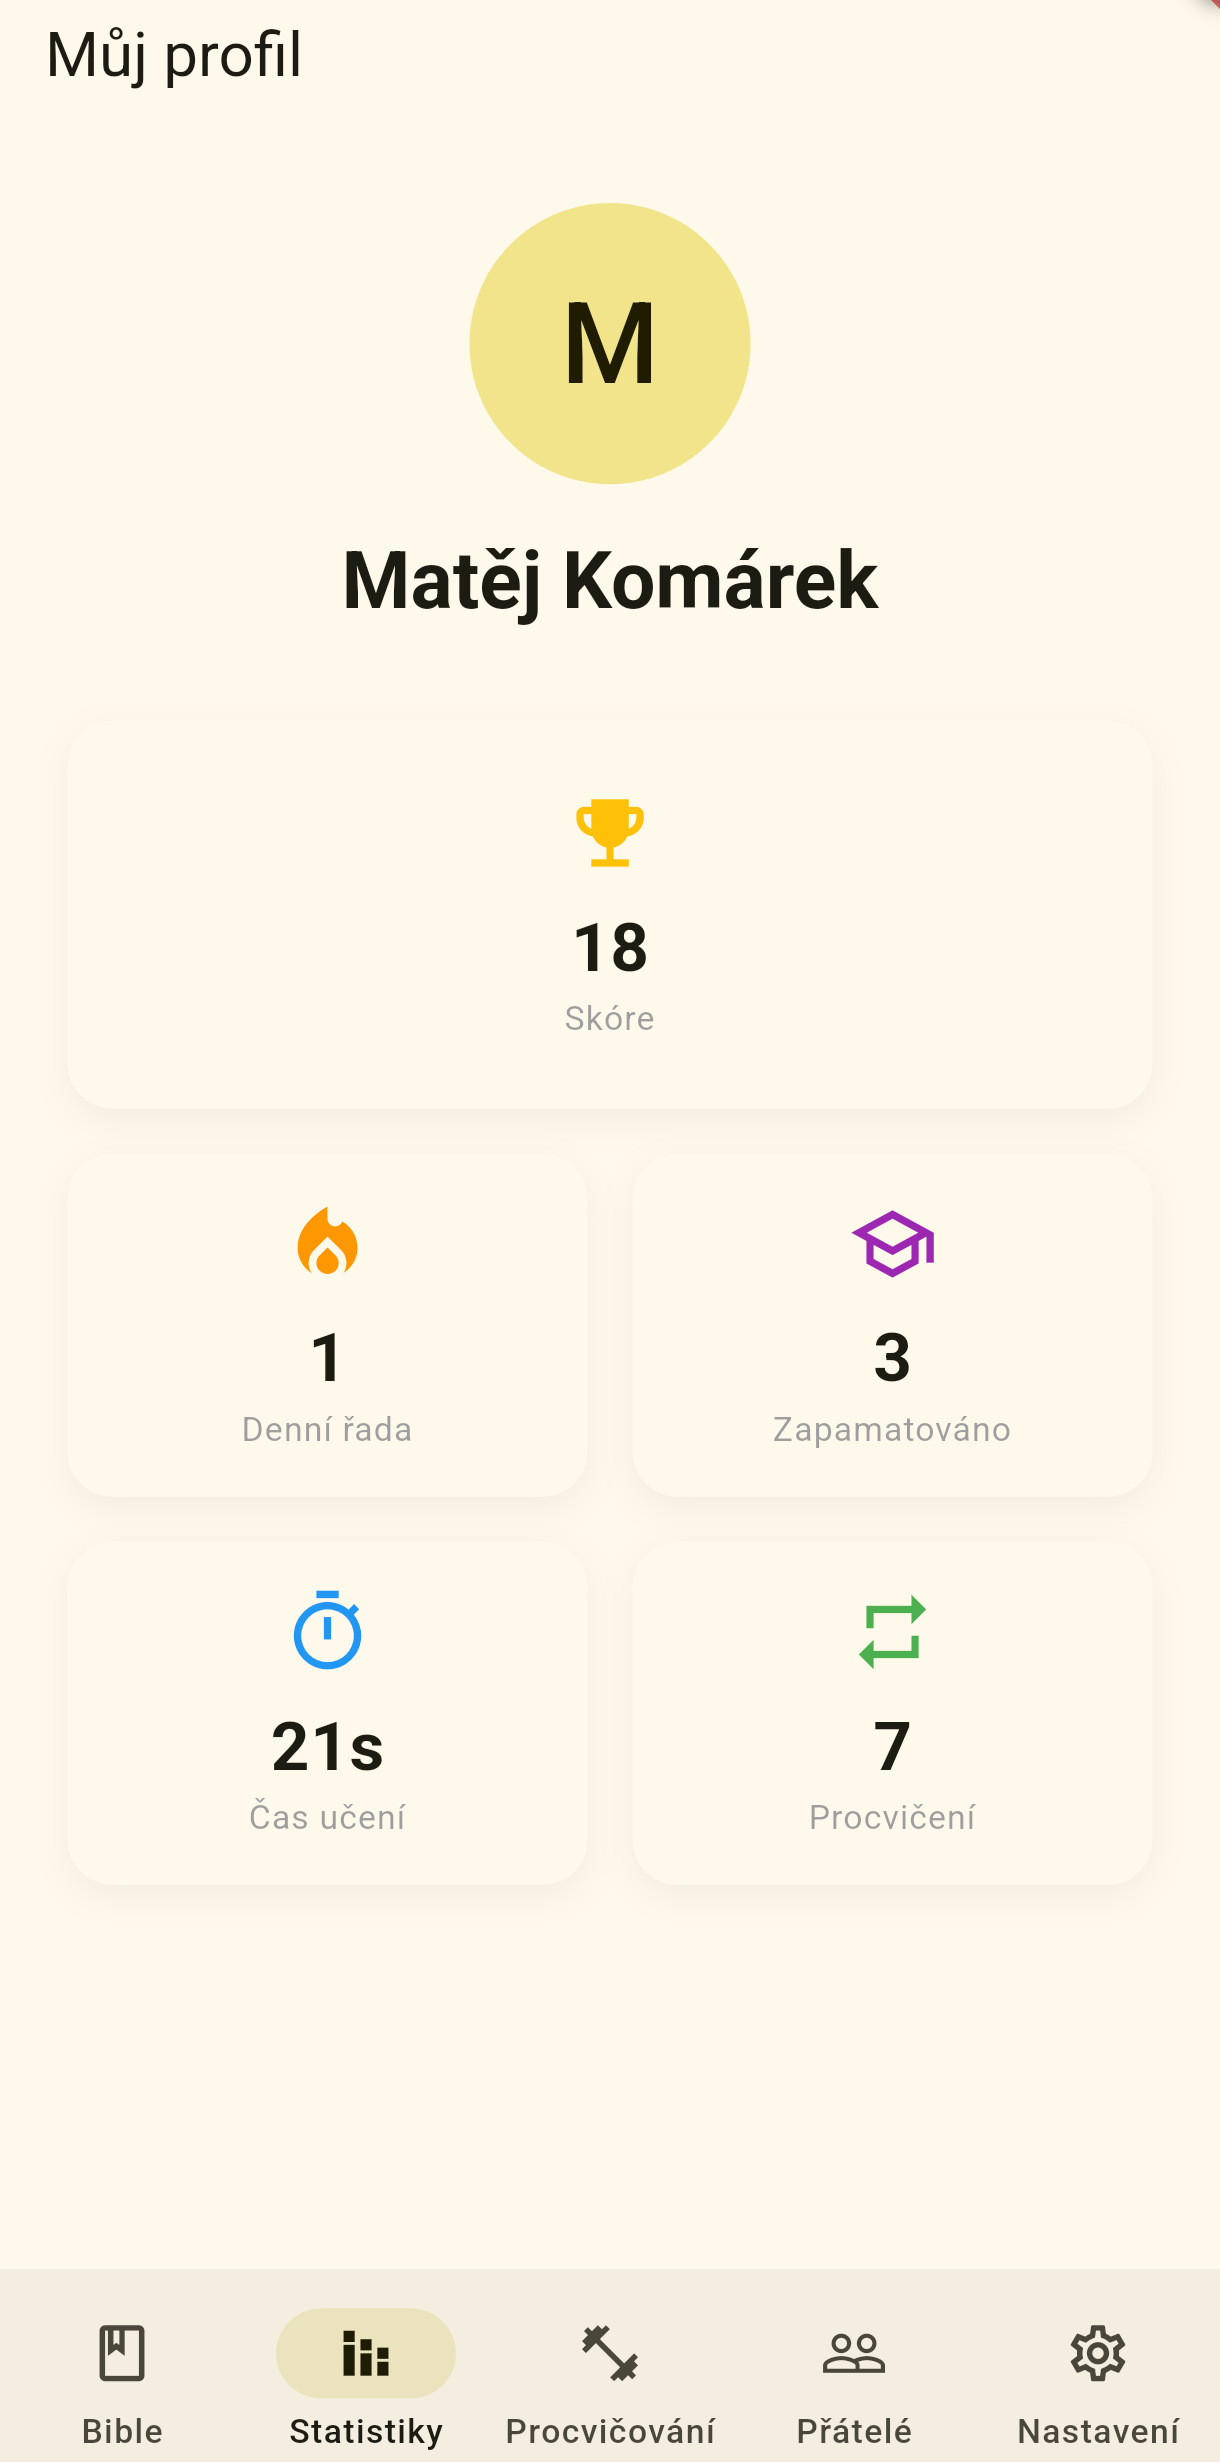
\includegraphics[height=12cm]{assets/screenshots/stats.png}
			\hspace{1cm}
			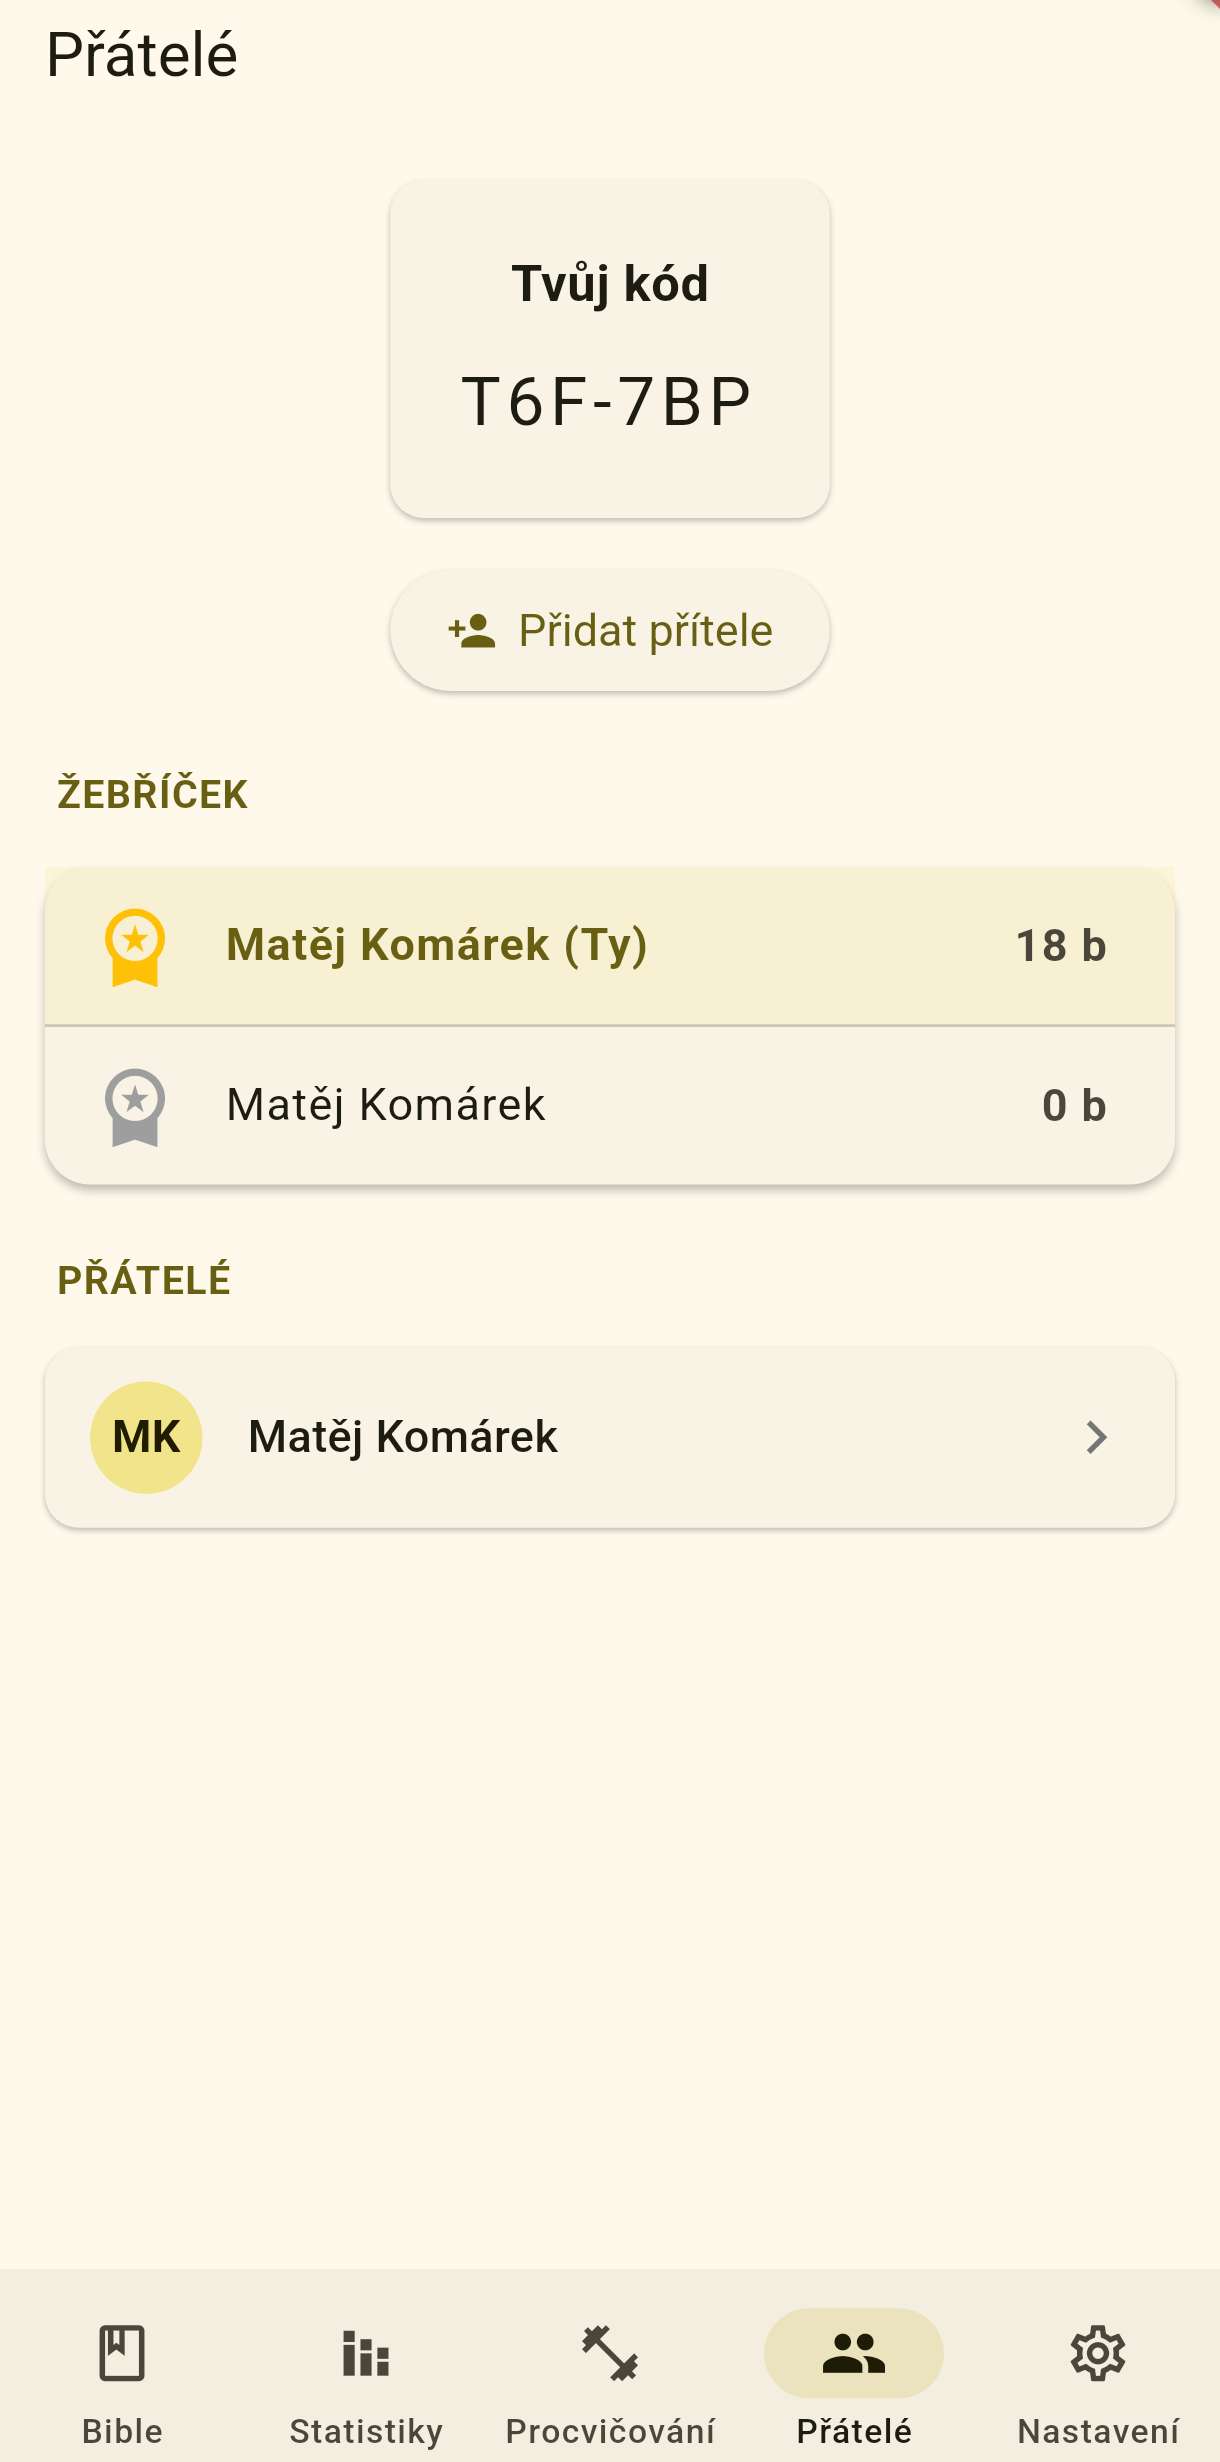
\includegraphics[height=12cm]{assets/screenshots/leaderboard.png}
			\caption{Osobní statistiky a žebříček přátel}
		\end{figure}
	\end{itemize}
	
	
	\newpage
	\section{Závěr}
	\subsection{Dosažené cíle a aktuální stav aplikace}
	
	\subsection{Dosažené cíle a aktuální stav aplikace}
	
	V rámci realizace maturitního projektu byla úspěšně navržena a implementována klientská mobilní aplikace i robustní serverová část. Výsledný systém Bible Memorizer v aktuálním stavu plně pokrývá veškeré funkční požadavky, přičemž klade mimořádný důraz na prvky gamifikace, které zvyšují uživatelskou retenci a efektivitu učení.
	
	Mezi klíčové dosažené milníky patří:
	\begin{itemize}
		\item \textbf{Implementace SM-2 algoritmu s herní smyčkou:} Jádrem aplikace je algoritmus intervalového opakování (Spaced Repetition), který je úzce propojen s herními mechanikami. Úspěšnost uživatele v minihrách (hodnocení $1$--$5$) přímo ovlivňuje obtížnost verše. Tento systém vytváří tzv. \textit{feedback loop}, kde je uživatel motivován k lepším výsledkům, aby mohl „postupovat“ v procesu zapamatování.
		\item \textbf{Systém denních řad (Streaks):} Pro posílení dlouhodobého návyku byl implementován mechanismus \textit{streak}, který vizuálně odměňuje uživatele za každodenní aktivitu. Tento psychologický prvek využívá principu averze ke ztrátě, kdy uživatel usiluje o udržení nepřerušené řady procvičování.
		\item \textbf{Sociální dynamika a žebříčky:} Aplikace obsahuje pokročilý sociální modul. Uživatelé mohou pomocí unikátních kódů navazovat přátelství a v reálném čase porovnávat své statistiky a skóre v žebříčcích. Tento prvek zdravé kompetice transformuje individuální učení v kolektivní zážitek.
		\item \textbf{Offline režim a synchronizace:} Aby nebyla herní smyčka přerušena nedostatkem konektivity, byl vyvinut synchronizační mechanismus využívající lokální databázi SQLite a serverový PostgreSQL. Postup uživatele, jeho skóre i dosažené úspěchy jsou bezpečně ukládány a při obnovení připojení automaticky synchronizovány pomocí časových razítek (\textit{timestamps}).
	\end{itemize}
	
	Aktuálně je aplikace ve stavu plně funkčního a otestovaného prototypu, který efektivně kombinuje vzdělávací cíle s principy herního designu.
	
	
	\subsection{Diskuze}
	
	\subsubsection{Zhodnocení splněných cílů}
	Lze konstatovat, že všechny hlavní cíle vytyčené v úvodní analýze a zadání projektu byly naplněny. Vytvořená platforma demonstruje funkční propojení moderních technologií (Flutter pro mobilní klient a NestJS pro backend) s vědeckými metodami učení. Důraz na gamifikaci a sledování denních řad efektivně přispívá k vyšší motivaci uživatelů.
	
	\subsection{Porovnání s konkurenčními řešeními}
	
	Ve srovnání s existujícími aplikacemi, které byly analyzovány v úvodu práce (VerseLocker, Bible Memory, Remember Me a BibleMe), přináší Bible Memorizer několik zásadních inovací a opravuje jejich největší nedostatky. 
	
	Jak shrnuje Tabulka \ref{tab:srovnani_aplikaci}, většina konkurence postrádá pokročilé metody učení. Zásadní výhodou naší aplikace je implementace intervalového opakování (SM-2), které u mnoha alternativ (např. VerseLocker či Remember Me) zcela chybí, což nutí uživatele spoléhat se na vlastní odhad toho, kdy si mají verš zopakovat. Na rozdíl od většiny konkurence také Bible Memorizer nevyžaduje manuální zadávání referencí do textových polí, což se v praxi ukázalo jako náchylné k chybám (u aplikace BibleMe to vedlo až k její nepoužitelnosti), ale nabízí integrovanou čtečku textu.
	
	Inovací prošel i sociální modul. Například aplikace VerseLocker sice žebříčky obsahuje, ale hodnotí pouze celkový počet „zapamatovaných“ veršů. Protože si tento stav určuje sám uživatel bez objektivního testování, je systém snadno zneužitelný a demotivační. Náš systém je spravedlivější, protože hodnotí skutečnou aktivitu v minihrách a udrženou denní řadu. V neposlední řadě Bible Memorizer jako jediný z testovaných plně podporuje české uživatelské rozhraní.
	
	\begin{table}[htbp]
		\centering
		\renewcommand{\arraystretch}{1.4} % Lehce zvětší výšku řádků pro lepší čitelnost
		\begin{tabular}{|l|c|c|c|c|}
			\hline
			\textbf{Aplikace} & \textbf{Intervalové opakov.} & \textbf{Čtečka Bible} & \textbf{Žebříčkek} & \textbf{České UI} \\
			\hline
			\hline
			\textbf{Bible Memorizer} & \textbf{Ano} & \textbf{Ano} & \textbf{Ano (Spravedlivý)} & \textbf{Ano} \\
			\hline
			Bible Memory & Ano & Ano & Ne & Ne \\
			\hline
			VerseLocker & Ne & Ne & Ano (Zavádějící)* & Ne \\
			\hline
			Remember Me & Ne & Ne & Ne & Ne** \\
			\hline
			BibleMe & Ne & Ne (Nefunkční) & Ne & Ne \\
			\hline
		\end{tabular}
		\caption{Srovnání funkcionality aplikace Bible Memorizer s existujícími řešeními}
		\label{tab:srovnani_aplikaci}
	\end{table}
	
	\footnotesize{
		\textit{* Žebříček v aplikaci VerseLocker hodnotí pouze počet veršů bez reálného testování znalostí. \\
			*** Aplikace Remember Me podporuje stažení českého překladu Bible, ale samotné rozhraní aplikace do češtiny přeloženo není.}
	}

	\subsection{Problémy během vývoje a jejich řešení}
	Největší technologickou výzvou během implementace byla obousměrná synchronizace dat mezi offline lokální databází (SQLite) a centrální serverovou databází (PostgreSQL. Zpočátku vyvstávala hrozba konfliktů při úpravě stejného záznamu na více zařízeních v offline režimu. Tento problém byl vyřešen zavedením robustního mechanismu založeného na časových razítkách (timestamps). Systém při slučování dat porovnává časová razítka a jako platný vždy přijímá ten nejnovější záznam.
	
	\subsection{Celkové shrnutí projektu}
	Cílem maturitního projektu bylo navrhnout a vyvinout mobilní aplikaci pro operační systém Android, která uživatelům pomůže zapamatovat si biblické verše efektivním a zároveň zábavným způsobem. Výsledkem je moderní, bezpečná a plně funkční platforma Bible Memorizer. Díky využití frameworku Flutter poskytuje aplikace plynulý uživatelský zážitek a konzistentní vzhled, zatímco backend postavený na NestJS zajišťuje spolehlivou synchronizaci a ochranu dat. Implementace gamifikačních prvků a algoritmu intervalového opakování pomáhá uživatelům dosahovat lepších výsledků s menším úsilím.
	
	\subsection{Možnosti budoucího rozvoje}
	Ačkoliv je aplikace v současném stavu plně použitelná, existuje zásadní prostor pro její další algoritmické vylepšení. Hlavním plánem do budoucna je nahrazení současného algoritmu SM-2 pokročilejším modelem HLR (Half-Life Regression). Tento model dokáže přesněji odhadovat pravděpodobnost zapomenutí konkrétního verše na základě širšího spektra proměnných a historie paměťových stop, což by vedlo k další optimalizaci intervalů opakování a celkovému zefektivnění procesu memorizace.
	
	% 8. Literatura
	\newpage
	\addcontentsline{toc}{section}{Literatura} % Adds to TOC manually
	
	\begin{thebibliography}{99}
		\bibitem{zdroj1} Citace
	\end{thebibliography}
	
	
	% 9. Seznam obrázků
	\newpage
	\listoffigures
	% \listoftables % Uncomment if you have tables
	
	
	% 10. Seznam příloh
	\newpage
	\section*{Seznam příloh}
	\addcontentsline{toc}{section}{Seznam příloh}
	\begin{itemize}
		\item \textbf{Příloha 1:} Use Case diagram a specifikace případů užití
		\item \textbf{Příloha 2:} UML Class diagram (Diagram tříd) backendu
	\end{itemize}
	
	
	% 11. Přílohy
	\newpage
	\section*{Přílohy}
	\addcontentsline{toc}{section}{Přílohy} % Přidá "Přílohy" do hlavního obsahu
	
	
	% TODO odkazat se
	% --- PŘÍLOHA 1 ---
	\subsection*{Příloha 1: Use Case diagram a specifikace případů užití}
	
	% Vložení samotného obrázku s diagramem. 
	% Parametr width=\textwidth zajistí, že se obří diagram smrskne přesně na šířku stránky.
	\begin{figure}[htbp]
		\centering
		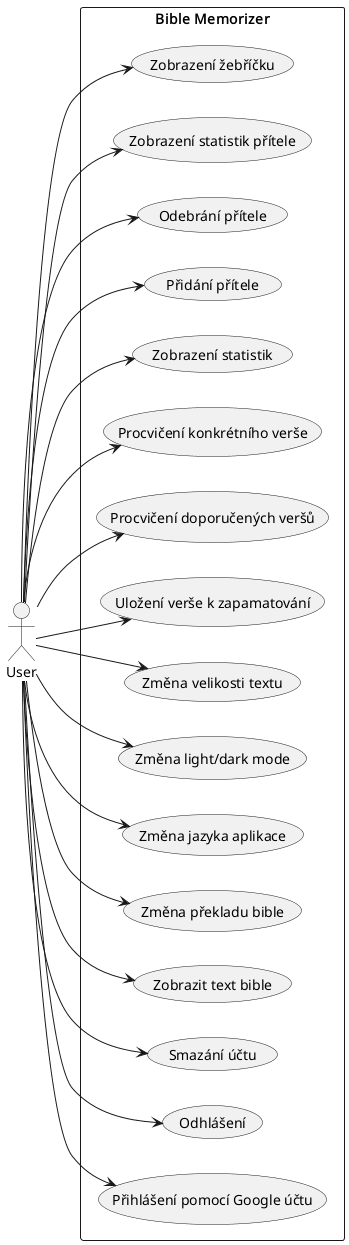
\includegraphics[height=0.73\textheight, keepaspectratio]{assets/usecase_diagram.png}
		\caption{Use Case diagram aplikace}
		\label{fig:use_case_diagram}
	\end{figure}
	
	\vspace{1cm}
	
	% TODO odkazat se
	% --- PŘÍLOHA 2 ---
	\newpage
	\subsection*{Příloha 2: UML Class diagram backendu}
	
	V této příloze je zobrazen detailní diagram tříd serverové části aplikace (NestJS). Diagram vizualizuje vnitřní strukturu kontrolerů, servisů a entit včetně jejich vzájemných vazeb a metod.
	
	\begin{figure}[htbp]
		\centering
		% width=\textwidth roztáhne diagram na šířku, 
		% height zajistí, aby nepřetekl výšku stránky
		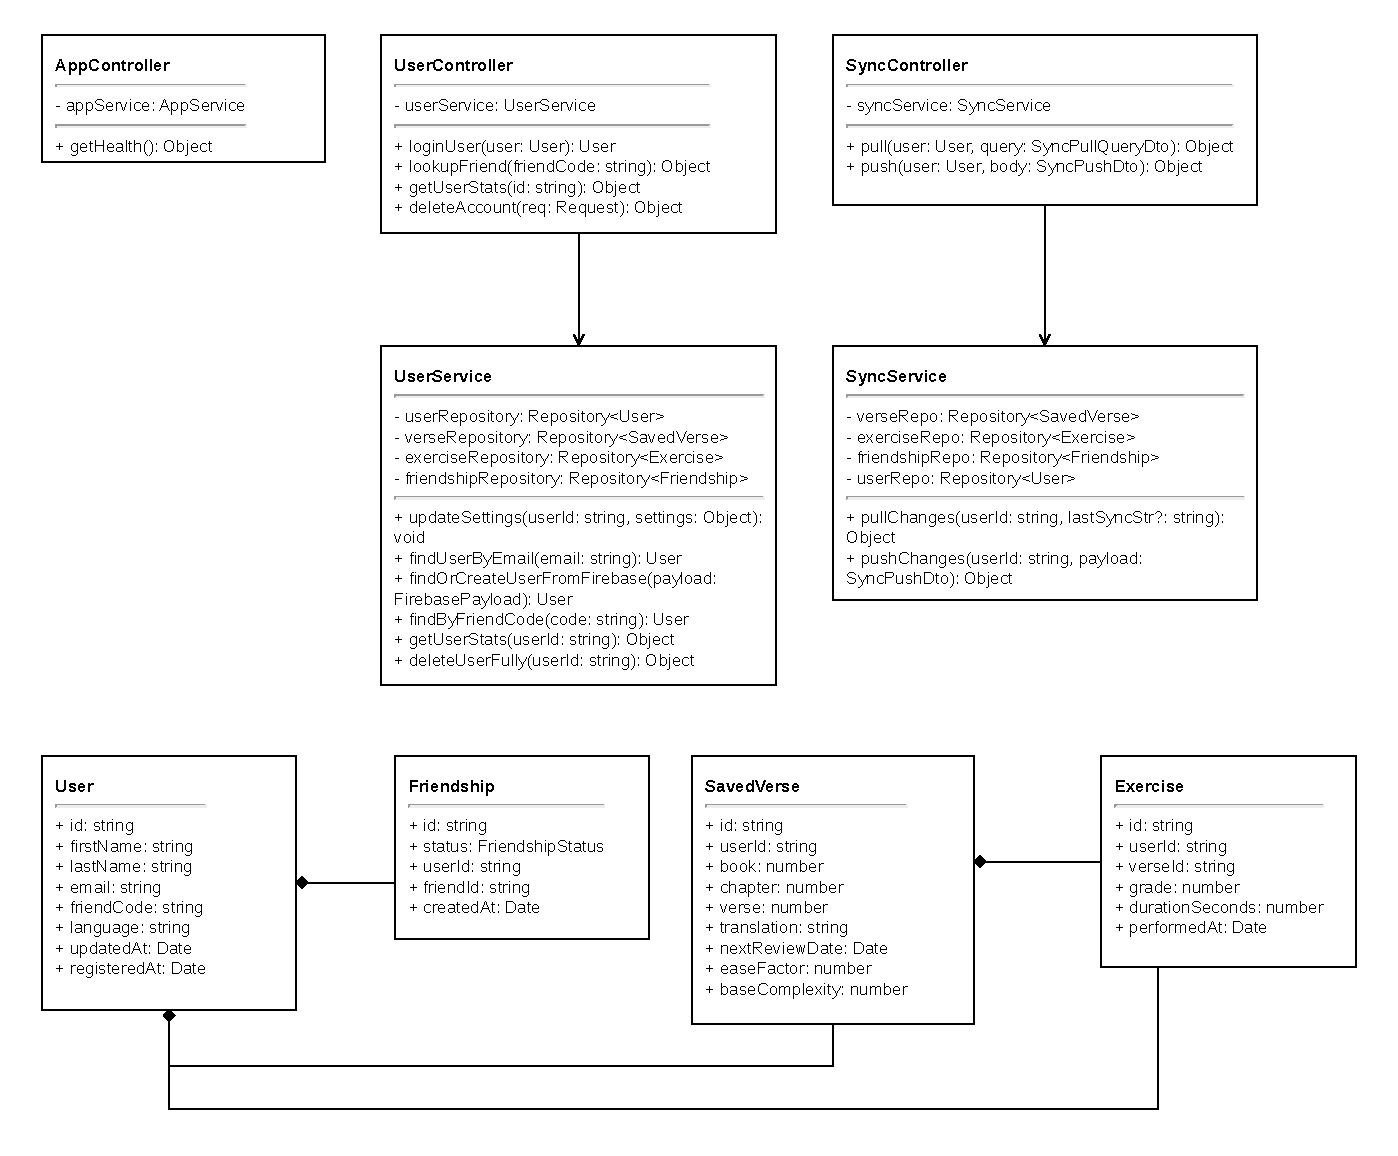
\includegraphics[width=\textwidth, height=0.85\textheight, keepaspectratio]{assets/class_diagram.pdf}
		\caption{Detailní architektura tříd systému Bible Memorizer}
		\label{fig:class_diagram_full}
	\end{figure}
	
\end{document}